% ============================================================================
% 4. Results
% ============================================================================
\section{Results}\label{sec:results}

\subsection{The completed three-stage programme}\label{sec:manifest}
The experimental programme is now complete and proceeds in three stages.
\emph{Stage 1} is the original GPU-scale study: a compact pre-LN encoder
($d_{\text{model}}=128$, 4 heads, $d_k=32$) trained on the full training
subsets (10{,}000 examples, 128-token sequences, batch 64) for 2 epochs, plus
the temperature ablation, an extended 25-epoch budget, and the original
language-modelling runs. \emph{Stage 2}, reported in this revision, completes
every grid that Stage 1 left open, on a documented replica protocol (2-core CPU
sandbox; 2{,}000-example training subsets, 64-token sequences, batch 32; full
specification in Sections~\ref{sec:replica-protocol}
and~S13 of the supplementary material): the 25-seed replica core, the corrected causal-mask
language-modelling grid (25 seeds $\times$ 3 variants), the head-dimension grid
$\dk \in \{32, 64, 128\}$, train-to-convergence with early stopping, and
multi-seed E1--E4 ablations. \emph{Stage 3}, also reported in this revision,
responds to the operating-point diagnosis of Section~\ref{sec:scale}: it
quantifies the regime in which the divisor can act at all (a power law,
validated by Monte Carlo), then deliberately moves the operating point into
that regime three ways~--- an injected logit gain, longer training at two head
dimensions, and inference-time divisor swaps in a pretrained decoder~--- and
adds the frontier stabilisers (QK-Norm, soft-capping) under which large logits
are tolerated in practice. All stages share the same matched-seed paired
design, statistical machinery, and analysis scripts.
In total the programme comprises 787 runs: 314 at GPU scale, 339 at replica
scale (312 pre-registered completions plus 27 mask-artifact probes), and 134
in the Stage-3 operating-point programme (128 matched-seed training runs plus
6 pretrained-model evaluations).

\begin{table}[t]
  \centering
  \caption{Completed experiment manifest. Stage 1 = GPU-scale protocol;
  Stage 2 = replica-scale completion; Stage 3 = operating-point programme
  (this revision). Every preregistered grid is complete in at least one
  stage.}
  \label{tab:manifest}
  \small
  \begin{tabular*}{\textwidth}{@{\extracolsep{\fill}} l l l r}
    \toprule
    \textbf{Grid} & \textbf{Design} & \textbf{Stage} & \textbf{Runs} \\
    \midrule
    Core classification & 3 variants $\times$ 25 seeds $\times$ 3 datasets & 1 & 225 \\
    Temperature ablation & 4 temperatures $\times$ 3 seeds $\times$ 2 datasets & 1 & 24 \\
    Extended budget & 3 variants $\times$ 5 seeds $\times$ 2 datasets, 25 epochs & 1 & 30 \\
    Core language modelling & 3 variants $\times$ 25 seeds (v1 protocol) & 1 & 25 \\
    Focused ablations E1--E4 & single-seed arms, 5 epochs & 1 & 10 \\
    \midrule
    Replica core classification & 3 variants $\times$ 25 seeds, AG News & 2 & 75 \\
    Replica language modelling & 3 variants $\times$ 25 seeds, corrected causal mask & 2 & 75 \\
    Head-dimension grid & $\dk \in \{32,64,128\}$ $\times$ 3 variants $\times$ 12 seeds & 2 & 108 \\
    Train-to-convergence & 3 variants $\times$ 5 seeds $\times$ 2 datasets, early stopping & 2 & 30 \\
    Replica ablations E1--E4 & 4 arms $\times$ 3 seeds $\times$ 2 datasets, 5 epochs & 2 & 24 \\
    Mask-artifact probes & leaky vs.\ causal, 3 and 10 epochs & 2 & 27 \\
    \midrule
    Logit-gain sweep & $g \in \{1,2,4,8,16,32\}$ $\times$ 3 variants $\times$ 4 seeds & 3 & 72 \\
    Regime-restored AG News & 6{,}000 train, 8 epochs, per-epoch probes, $\dk \in \{32,128\}$ & 3 & 18 \\
    Frontier-stabiliser bridge & QK-Norm / soft-cap arms $\times$ 4 seeds & 3 & 20 \\
    LM logit gain & $g \in \{1,4\}$ $\times$ 3 variants $\times$ 3 seeds, seq 128 & 3 & 18 \\
    Frontier divisor swap & GPT-2 + GPT-2-medium, inference-time, 3 divisors & 3 & 6 \\
    \midrule
    \textbf{Total} & & & \textbf{787} \\
    \bottomrule
  \end{tabular*}
\end{table}

\subsection{Stage 1: GPU-scale core comparison}\label{sec:main-results}
Figure~\ref{fig:main} and Table~\ref{tab:core} present test accuracy across the
25-seed core grid. On AG News, standard scaling reached 91.23\% ($\pm 0.25$),
versus 91.13\% ($\pm 0.26$) for the temperature variant $\tau = 2$ and 90.92\%
($\pm 0.32$) for $1/\dk$~--- a strictly ordered pattern in which softening the
attention distribution monotonically hurt. On the binary sentiment tasks the
ordering vanished: SST-2 accuracies fell within 0.08\,\pp{} of one another and
IMDB accuracies within 0.04\,\pp, with overlapping seed distributions
(Figure~\ref{fig:main}, middle and right).

\begin{figure}[t]
  \centering
  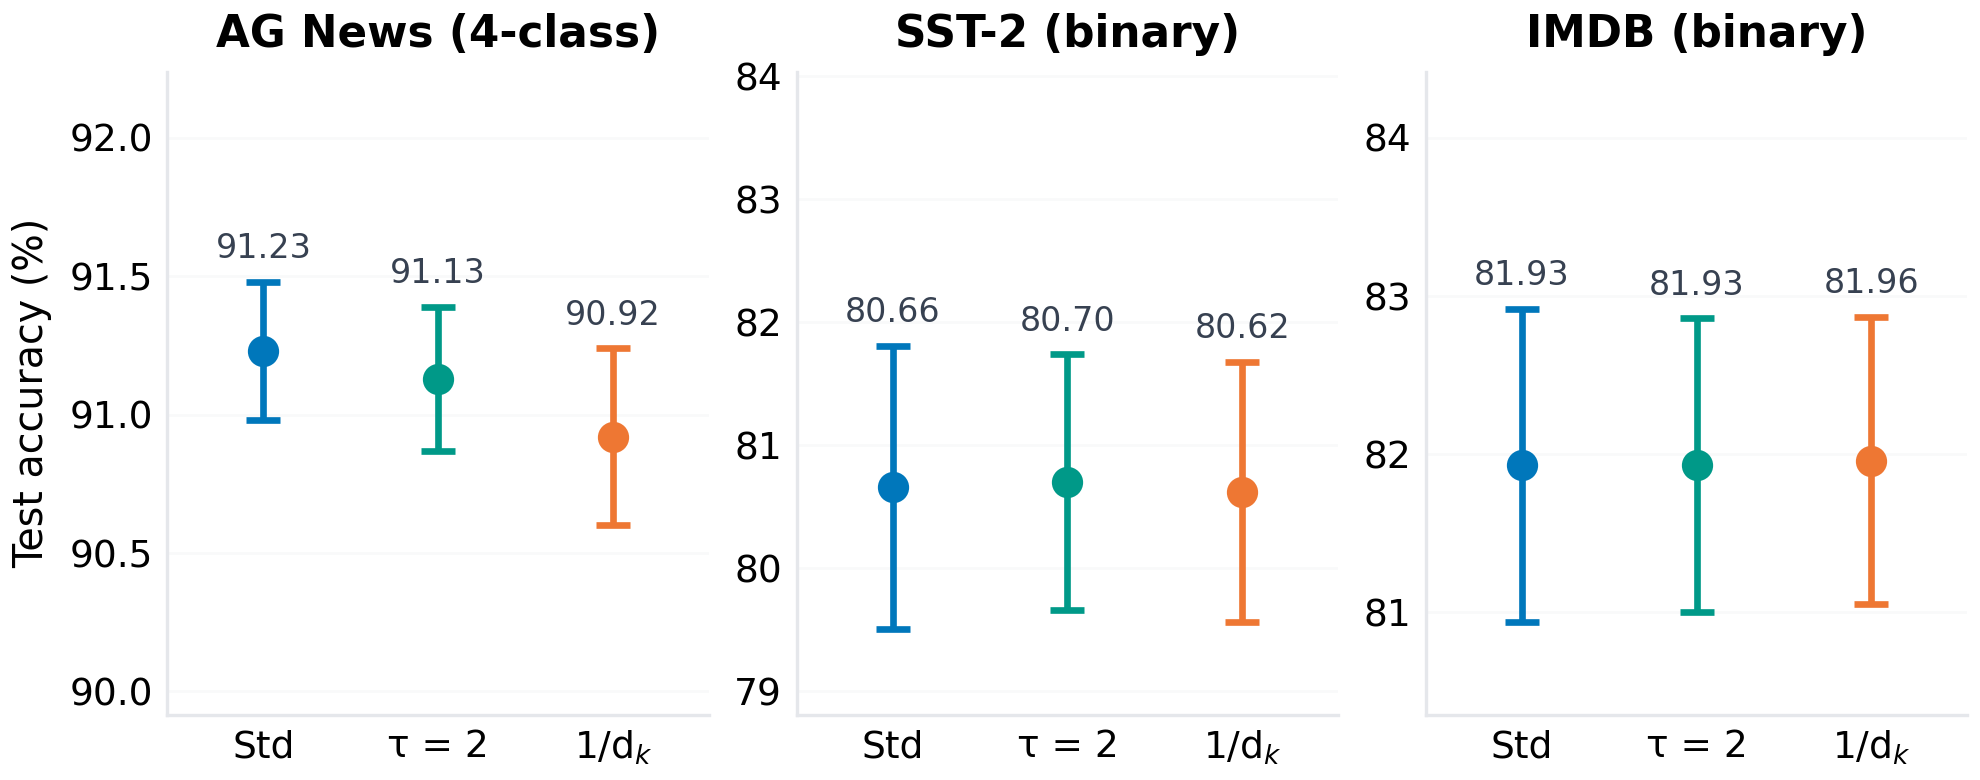
\includegraphics[width=\textwidth]{figures/fig_main_performance.png}
  \caption{Core-grid test accuracy (mean $\pm$ one standard deviation across 25
  matched seeds, 2-epoch budget). Only AG News shows a strictly ordered, visibly
  separated pattern; on SST-2 and IMDB the seed distributions overlap almost
  completely.}
  \label{fig:main}
\end{figure}

\begin{table}[t]
  \centering
  \caption{Core-grid results, Stage 1 (25 matched seeds, 2-epoch GPU budget;
  language-modelling rows are the superseded v1 leaky-mask values, see
  Section~\ref{sec:lm}). $\pm$ denotes one standard deviation across seeds;
  CI is the 95\% confidence interval of the mean.}
  \label{tab:core}
  \small
  \begin{tabular*}{\textwidth}{@{\extracolsep{\fill}} l l r r c r}
    \toprule
    \textbf{Dataset} & \textbf{Variant} & \textbf{Mean} & \textbf{$\pm$ SD} &
    \textbf{95\% CI} & \textbf{$n$} \\
    \midrule
    \multirow{3}{*}{AG News (\%)} & Standard & 91.23 & 0.25 & $[91.13, 91.33]$ & 25 \\
      & Temp ($\tau=2$) & 91.13 & 0.26 & $[91.03, 91.24]$ & 25 \\
      & $1/\dk$ & 90.92 & 0.32 & $[90.80, 91.04]$ & 25 \\
    \midrule
    \multirow{3}{*}{SST-2 (\%)} & Standard & 80.66 & 1.15 & $[80.19, 81.13]$ & 25 \\
      & Temp ($\tau=2$) & 80.70 & 1.04 & $[80.27, 81.13]$ & 25 \\
      & $1/\dk$ & 80.62 & 1.06 & $[80.18, 81.06]$ & 25 \\
    \midrule
    \multirow{3}{*}{IMDB (\%)} & Standard & 81.93 & 0.99 & $[81.52, 82.34]$ & 25 \\
      & Temp ($\tau=2$) & 81.93 & 0.93 & $[81.55, 82.31]$ & 25 \\
      & $1/\dk$ & 81.96 & 0.91 & $[81.58, 82.34]$ & 25 \\
    \midrule
    \multirow{3}{*}{WikiText-2 (ppl $\downarrow$, v1 artefact$^\dagger$)} & Standard & 1.0917 & 0.0061 & $[1.089, 1.095]$ & 15 \\
      & Temp ($\tau=2$) & 1.0882 & 0.0056 & $[1.083, 1.093]$ & 7 \\
      & $1/\dk$ & 1.0809 & 0.0021 & $[1.077, 1.085]$ & 3 \\
    \bottomrule
    \multicolumn{6}{l}{\footnotesize $^\dagger$Historical v1 values under the leaky (non-causal) mask; superseded by the corrected
    protocol in Table~\ref{tab:lm}.}
  \end{tabular*}
\end{table}

\subsection{Paired differences and effect sizes (Stage 1)}\label{sec:paired}
Because the design is seed-matched, the informative statistics are the paired
differences of Table~\ref{tab:paired} and Figure~\ref{fig:paired}. On AG News,
standard scaling beat $1/\dk$ by $+0.31$\,\pp{} (95\% CI $[0.22, 0.39]$, $d_z =
1.52$, $t(24) = 7.60$, $p_{\text{Holm}} < 0.001$) and beat $\tau = 2$ by
$+0.10$\,\pp{} (95\% CI $[0.02, 0.17]$, $d_z = 0.53$, $t(24) = 2.65$,
$p_{\text{Holm}} = 0.013$)~--- large and medium paired effect sizes
respectively \cite{cohen1988}. Wilcoxon signed-rank tests confirmed both
directions. On SST-2 and IMDB all four comparisons had confidence intervals
straddling zero and negligible effect sizes ($|d_z| \le 0.19$,
$p_{\text{Holm}} \ge 0.70$). In other words, the AG News effect is not an
artefact of seed luck: it appears in the matched within-seed contrasts, where
initialization and data order are held constant.

\begin{table}[t]
  \centering
  \caption{Paired statistics versus the standard baseline (unit: within-seed
  difference, $n = 25$). Positive differences favour standard scaling.
  $p_{\text{Holm}}$ is Holm--Bonferroni corrected across the two comparisons
  within each dataset. Significance codes: $^{***}\,p < 0.001$,
  $^{*}\,p < 0.05$ after correction.}
  \label{tab:paired}
  \small
  \begin{tabular*}{\textwidth}{@{\extracolsep{\fill}} l l c c c c c c}
    \toprule
    \textbf{Dataset} & \textbf{Comparison} & \textbf{$\Delta$ (pp)} &
    \textbf{95\% CI (pp)} & \textbf{$d_z$} & \textbf{$t(24)$} &
    \textbf{$p_{\text{Holm}}$} & \textbf{Sig.} \\
    \midrule
    AG News & $1/\dk$ vs.\ std & $+0.31$ & $[+0.22, +0.39]$ & $1.52$ & $7.60$ & $<0.001$ & $^{***}$ \\
            & $\tau=2$ vs.\ std & $+0.10$ & $[+0.02, +0.17]$ & $0.53$ & $2.65$ & $0.013$ & $^{*}$ \\
    \midrule
    SST-2   & $1/\dk$ vs.\ std & $+0.04$ & $[-0.23, +0.31]$ & $0.06$ & $0.30$ & $0.781$ & \\
            & $\tau=2$ vs.\ std & $-0.05$ & $[-0.31, +0.21]$ & $-0.07$ & $-0.35$ & $0.718$ & \\
    \midrule
    IMDB    & $1/\dk$ vs.\ std & $-0.04$ & $[-0.11, +0.04]$ & $-0.19$ & $-0.95$ & $0.703$ & \\
            & $\tau=2$ vs.\ std & $-0.01$ & $[-0.06, +0.05]$ & $-0.04$ & $-0.20$ & $0.831$ & \\
    \bottomrule
  \end{tabular*}
\end{table}

\begin{figure}[t]
  \centering
  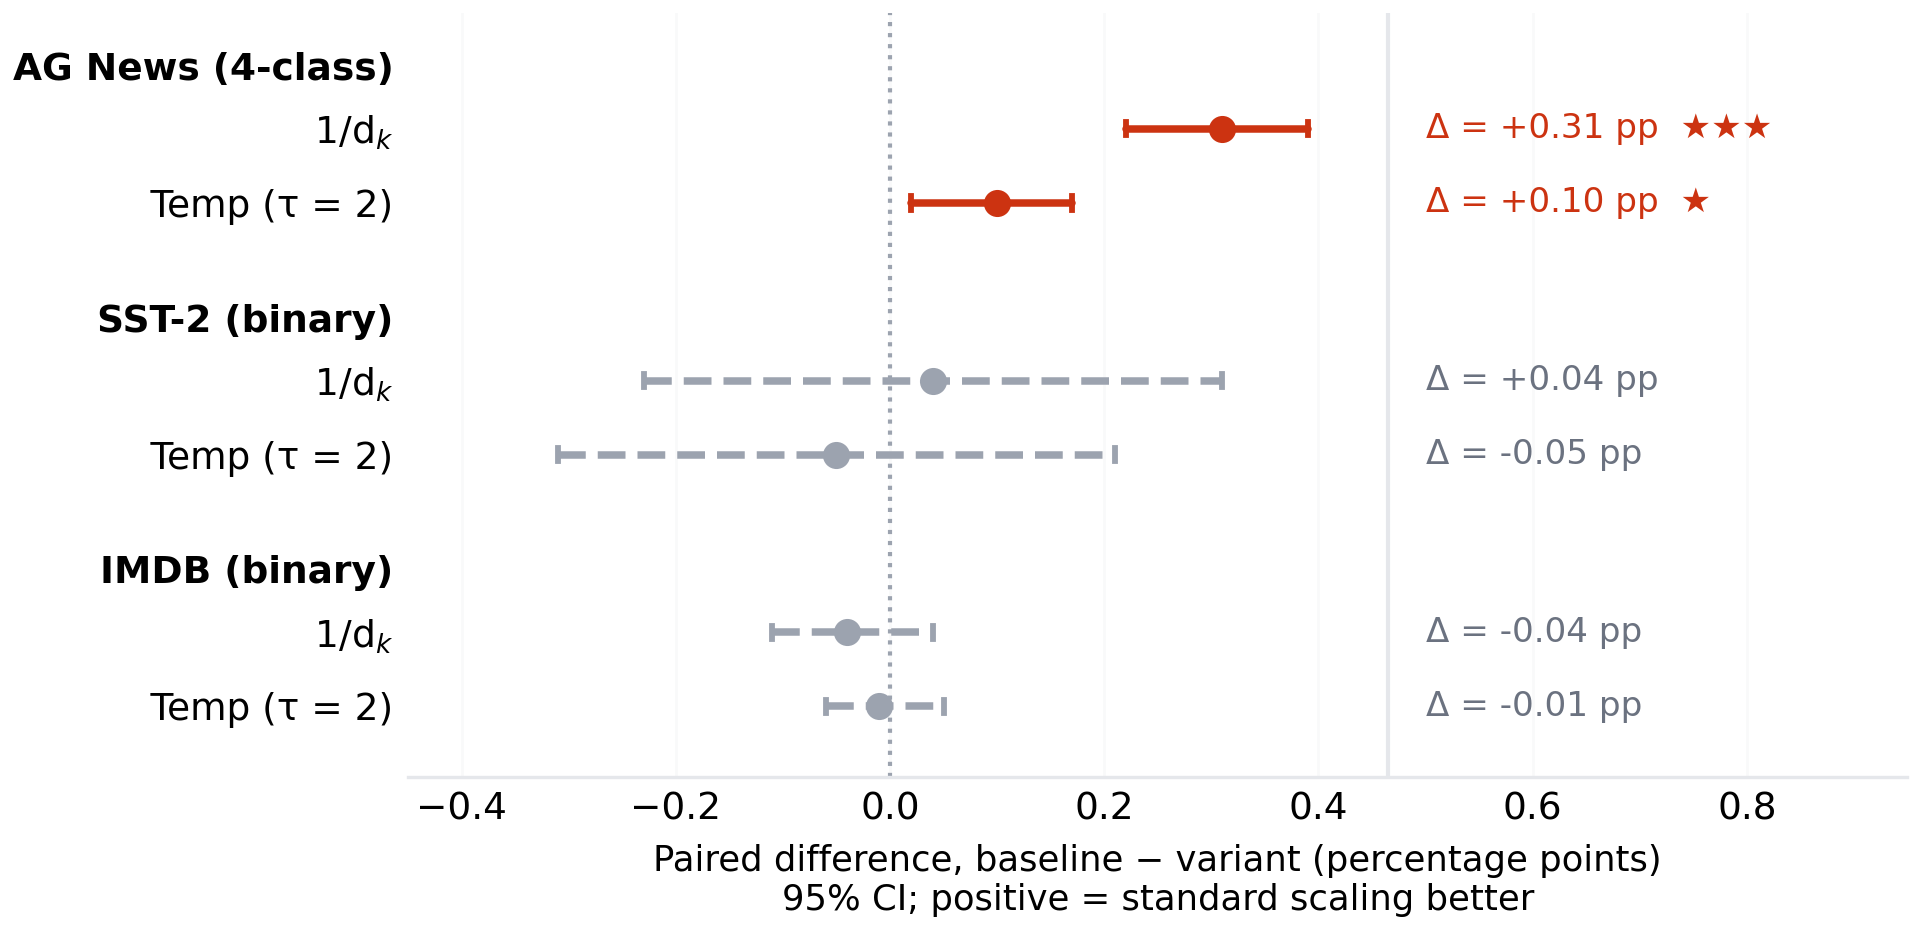
\includegraphics[width=0.96\textwidth]{figures/fig_paired_differences.png}
  \caption{Seed-matched paired differences with 95\% confidence intervals.
  Only the two AG News comparisons (red) exclude zero after Holm--Bonferroni
  correction; all SST-2 and IMDB intervals (grey) straddle zero.}
  \label{fig:paired}
\end{figure}

\subsection{Stage 2: replica completion of the core grid}\label{sec:replica}
The first Stage-2 question is whether the AG News effect of Section~\ref{sec:paired}
survives a fivefold reduction in training data and sequence length. Under the
replica protocol (2{,}000 training examples, 64-token sequences, otherwise
identical architecture and matched-seed design), all three variants land within
0.01\,\pp{} of one another: 78.51\% ($\pm 1.26$) for standard scaling, 78.51\%
($\pm 1.25$) for $\tau = 2$, and 78.50\% ($\pm 1.24$) for $1/\dk$
(Figure~\ref{fig:replica}a, Table~\ref{tab:replica}). The paired differences
are $-0.01$\,\pp{} (95\% CI $[-0.04, +0.02]$, $d_z = -0.13$) for $1/\dk$ versus
standard and $+0.00$\,\pp{} ($d_z = 0.04$) for $\tau=2$ versus standard; both
$p_{\text{Holm}} = 1.00$ (Figure~\ref{fig:replica}b). The Stage-1 AG News
effect of $+0.31$\,\pp{} therefore does \emph{not} replicate at this operating
point: the replica confidence interval excludes any advantage larger than
0.02\,\pp. We return to the interpretation of this scale dependence in
Section~\ref{sec:scale}.

\begin{figure}[t]
  \centering
  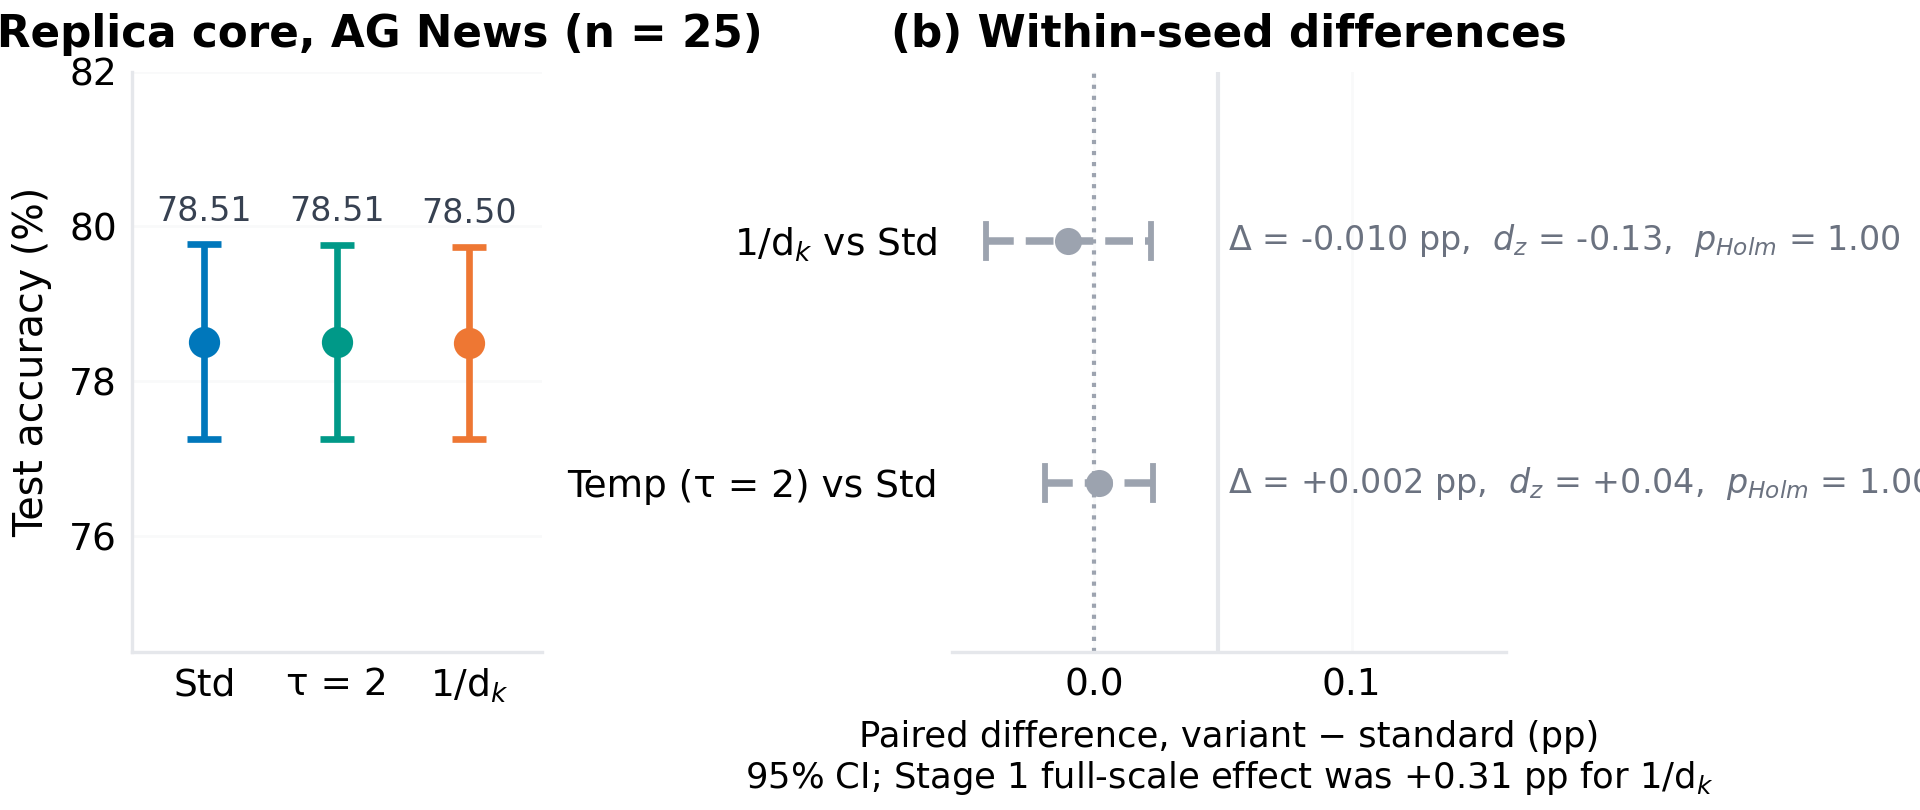
\includegraphics[width=\textwidth]{figures/fig_stage2_core.png}
  \caption{Stage-2 replica core on AG News (25 matched seeds, 2 epochs).
  (a) Test accuracy by variant. (b) Within-seed paired differences with 95\%
  CIs; both intervals straddle zero, and the replica CI excludes the Stage-1
  full-scale effect of $+0.31$\,\pp{} for $1/\dk$.}
  \label{fig:replica}
\end{figure}

\begin{table}[t]
  \centering
  \caption{Stage-2 replica results. Left: AG News core (25 seeds, 2 epochs).
  Right: within-seed paired statistics versus standard ($n=25$);
  $p_{\text{Holm}}$ across the two comparisons.}
  \label{tab:replica}
  \small
  \begin{tabular*}{\textwidth}{@{\extracolsep{\fill}} l r r r l}
    \toprule
    \textbf{Variant} & \textbf{Mean (\%)} & \textbf{$\pm$ SD} & \textbf{$n$} &
    \textbf{Paired vs.\ standard} \\
    \midrule
    Standard & 78.51 & 1.26 & 25 & --- \\
    Temp ($\tau=2$) & 78.51 & 1.25 & 25 & $\Delta = +0.00$ pp, $d_z = 0.04$, $p_{\text{Holm}} = 1.00$ \\
    $1/\dk$ & 78.50 & 1.24 & 25 & $\Delta = -0.01$ pp, $d_z = -0.13$, $p_{\text{Holm}} = 1.00$ \\
    \bottomrule
  \end{tabular*}
\end{table}

\subsection{Stage 2: head-dimension grid ($\dk \in \{32, 64, 128\}$)}\label{sec:grid}
The variance argument behind $\sqrt{\dk}$ \cite{vaswani2017} predicts that the
logit standard deviation grows as $\sqrt{\dk}$ when the divisor is held at its
standard value but as $\dk$ when the divisor is $1/\dk$; the mismatch between
the two scalings should therefore \emph{amplify} with head dimension, making
larger $\dk$ the regime where the 2017 default is most likely to matter. We
tested this directly on AG News with $d_{\text{model}} = 128$ and
$n_{\text{heads}} \in \{4, 2, 1\}$, giving $\dk \in \{32, 64, 128\}$, 3 variants
$\times$ 12 seeds per point (Table~\ref{tab:grid}, Figure~\ref{fig:grid}).
The prediction is not borne out at this operating point: the $1/\dk$-versus-standard
gap is $+0.010$\,\pp{} ($p = 0.63$) at $\dk=32$, $+0.008$\,\pp{} ($p = 0.75$) at
$\dk=64$, and $+0.017$\,\pp{} ($p = 0.56$) at $\dk=128$, and the paired change in
the gap between $\dk=128$ and $\dk=32$ is $-0.006$\,\pp{} (95\% CI $[-0.077,
+0.064]$, $p = 0.85$). The same holds for $\tau = 2$. The mechanism is
measurable: at this scale the trained models' \emph{raw} logit standard
deviation is of order 1 (1.02--1.19 across variants; Section~\ref{sec:diagnostics}),
so after division by $\sqrt{\dk} \in \{5.7, 8, 11.3\}$ or by $\dk \in \{32, 64,
128\}$ every variant operates in the softmax's near-uniform regime, where
rescaling the logits changes almost nothing downstream. The theoretical
amplification only bites once raw logit variance grows past the divisor, which
the Stage-1 full-data protocol approaches but the replica does not.

\begin{figure}[t]
  \centering
  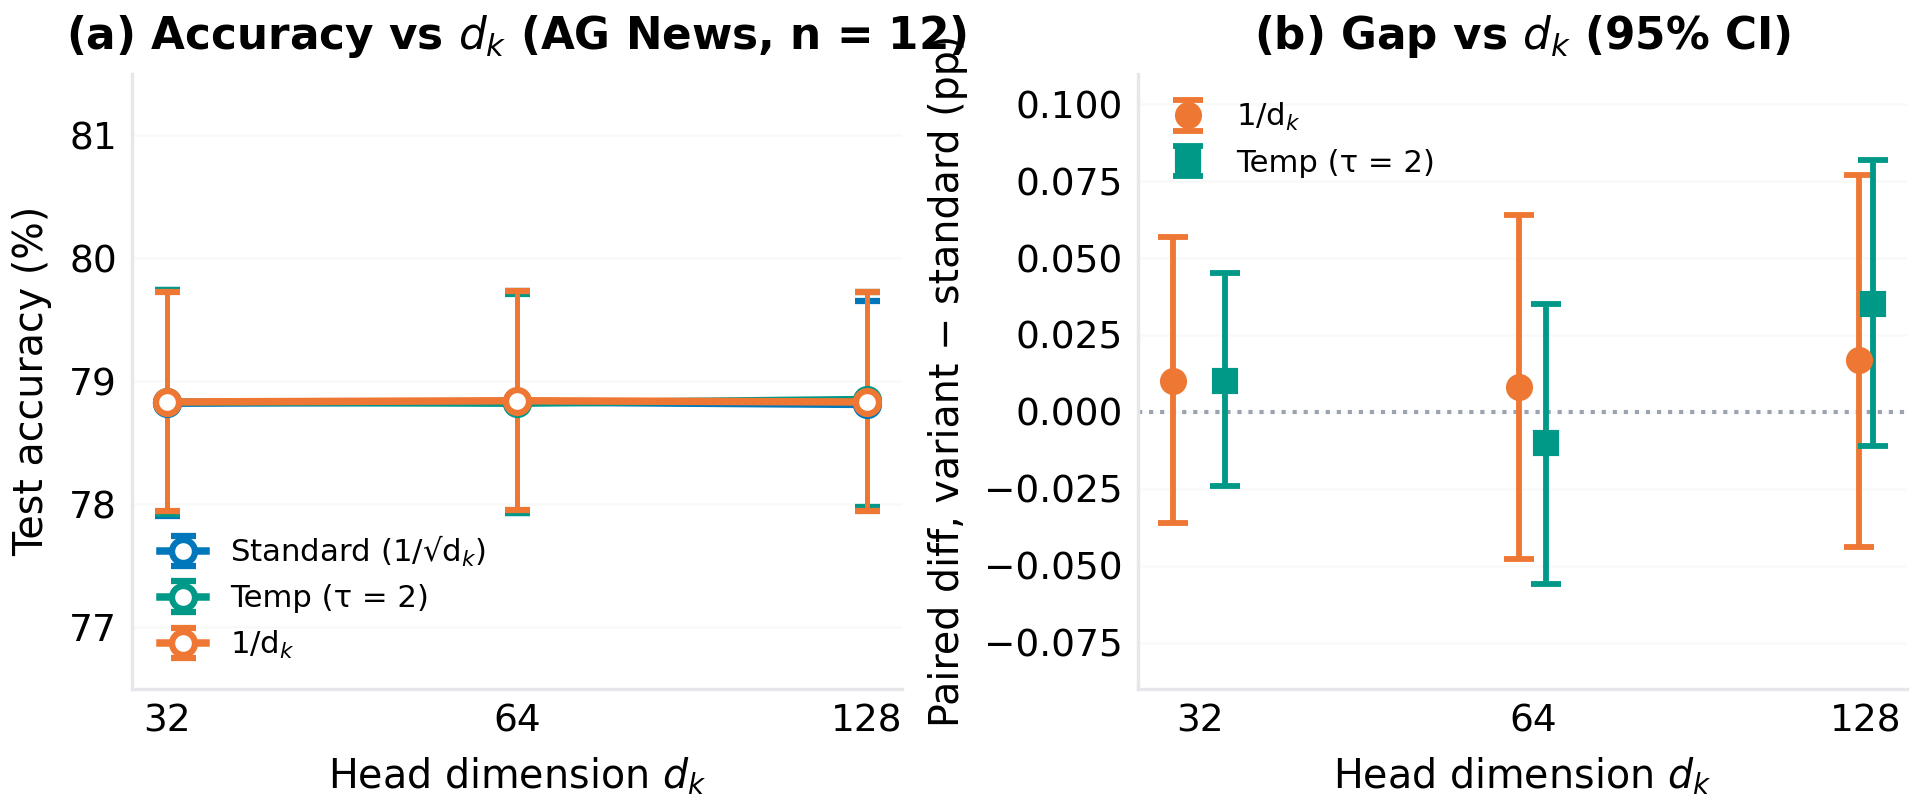
\includegraphics[width=\textwidth]{figures/fig_dk_grid.png}
  \caption{Head-dimension grid on AG News (12 matched seeds per point).
  (a) Test accuracy versus $\dk$ for the three variants. (b) Within-seed gap
  versus standard with 95\% CIs; no trend with $\dk$ (trend $p = 0.85$).}
  \label{fig:grid}
\end{figure}

\begin{table}[t]
  \centering
  \caption{Head-dimension grid, AG News replica (mean $\pm$ SD over 12 seeds;
  within-seed paired differences versus standard).}
  \label{tab:grid}
  \small
  \begin{tabular*}{\textwidth}{@{\extracolsep{\fill}} c c c c c c}
    \toprule
    \textbf{$\dk$} & \textbf{Std (\%)} & \textbf{$\tau{=}2$ (\%)} &
    \textbf{$1/\dk$ (\%)} & \textbf{$\Delta(\tau{=}2)$ (pp)} &
    \textbf{$\Delta(1/\dk)$ (pp)} \\
    \midrule
    32  & 78.82 $\pm$ 0.92 & 78.83 $\pm$ 0.91 & 78.83 $\pm$ 0.89 &
    $+0.01$ ($p{=}0.52$) & $+0.01$ ($p{=}0.63$) \\
    64  & 78.83 $\pm$ 0.90 & 78.82 $\pm$ 0.89 & 78.84 $\pm$ 0.89 &
    $-0.01$ ($p{=}0.63$) & $+0.01$ ($p{=}0.75$) \\
    128 & 78.81 $\pm$ 0.84 & 78.85 $\pm$ 0.87 & 78.83 $\pm$ 0.89 &
    $+0.04$ ($p{=}0.12$) & $+0.02$ ($p{=}0.56$) \\
    \bottomrule
  \end{tabular*}
\end{table}

\subsection{Temperature ablation (Stage 1)}\label{sec:temp-ablation}
The preregistered temperature sweep ($\tau \in \{0.5, 1.0, 1.5, 2.0\}$, 3 seeds
per point, 2 epochs) probes the direction of the effect around the standard
point (Figure~\ref{fig:temp}, Table~\ref{tab:temp}). On SST-2, sharper attention
was monotonically (if noisily) better: $\tau = 0.5$ reached 82.31\% versus
80.77\% for $\tau = 2$~--- a 1.54\,\pp{} spread~--- and on IMDB $\tau = 0.5$
again produced the highest mean (82.29\%), although the $\tau$-response was
flatter. Standard scaling ($\tau = 1$) was intermediate on both datasets. These
3-seed observations are exploratory: confidence intervals are wide (up to
$\pm 1.04$\,\pp{} on SST-2 $\tau = 1.5$), so the sharpest temperature's lead
over the 25-seed core-grid baselines (about $+1.6$\,\pp{} on SST-2) should be
treated as a promising direction rather than an established effect. The
directional pattern is nonetheless consistent with the distillation literature,
where lower temperatures sharpen attention and can help tasks that require
focused token selection \cite{zhang2022temp,hinton2015}.

\begin{figure}[t]
  \centering
  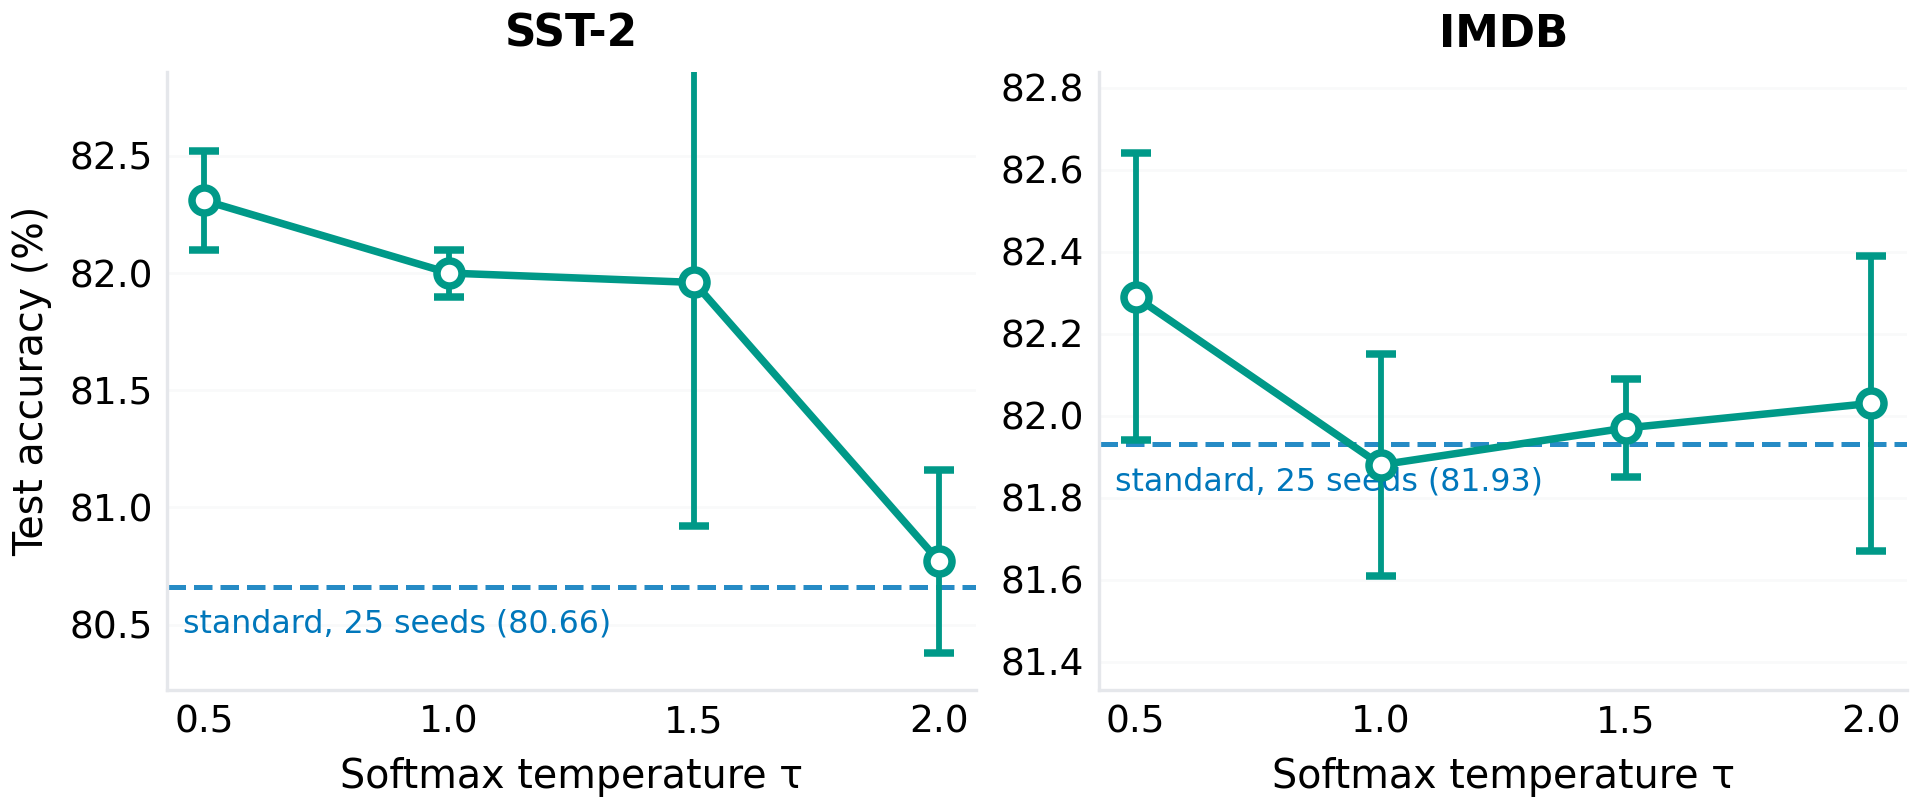
\includegraphics[width=0.9\textwidth]{figures/fig_temperature_ablation.png}
  \caption{Temperature ablation ($n = 3$ seeds per point, 2 epochs; error bars:
  $\pm$ one standard deviation). Dashed reference lines show the 25-seed core
  standard-scaling result at $\tau = 1$.}
  \label{fig:temp}
\end{figure}

\begin{table}[t]
  \centering
  \caption{Temperature ablation results (mean $\pm$ SD across 3 seeds).}
  \label{tab:temp}
  \small
  \begin{tabular*}{0.8\textwidth}{@{\extracolsep{\fill}} l c c c c}
    \toprule
    \textbf{$\tau$} & \textbf{SST-2 (\%)} & \textbf{SD} & \textbf{IMDB (\%)} & \textbf{SD} \\
    \midrule
    0.5 & \textbf{82.31} & 0.21 & \textbf{82.29} & 0.35 \\
    1.0 & 82.00 & 0.10 & 81.88 & 0.27 \\
    1.5 & 81.96 & 1.04 & 81.97 & 0.12 \\
    2.0 & 80.77 & 0.39 & 82.03 & 0.36 \\
    \bottomrule
  \end{tabular*}
\end{table}

\subsection{Training-budget sensitivity and train-to-convergence}\label{sec:budget}
If the AG News-scale differences reflect early-training dynamics rather than a
permanent quality gap, they should shrink with longer training. The Stage-1
extended grid (5 seeds, 25 epochs, checkpoints at 2/5/10/25) supports this on
the binary tasks: all three variants converge to approximately 84\% on SST-2 and
84.5\% on IMDB, and the variant differences at 25 epochs ($\le 0.2$\,\pp) are
within seed noise (Figure~\ref{fig:curves}). The variants' curves are nearly
parallel and interleave across checkpoints~--- underpowered (5 seeds) but
consistent with the early-training interpretation, and with the observation of
Zhai et al. \cite{zhai2023} that attention-entropy differences between
configurations diminish as training progresses.

Stage 2 replaces the fixed 2-epoch cut-off with train-to-convergence: 5 seeds
per variant on SST-2 and IMDB, up to 20 epochs, model selection by validation
loss with a patience of 3 epochs (Figure~\ref{fig:conv}, Table~\ref{tab:conv}).
Validation loss bottoms at epoch $\approx 2$ for every variant on both datasets
(mean best epoch 2.2 on SST-2 and 1.6 on IMDB), early stopping halts training at
epochs 5--6, and the best-validation checkpoints differ by at most $+0.07$\,\pp
between variants ($p \ge 0.31$). The learning curves of the three variants are
visually indistinguishable at every epoch: neither the asymptotic accuracy nor
the convergence speed depends on the scaling function in this regime. The
answer to whether the divisor affects asymptote or speed is therefore ``neither
-- at this operating point the entire training trajectory is divisor-invariant''.

\begin{figure}[t]
  \centering
  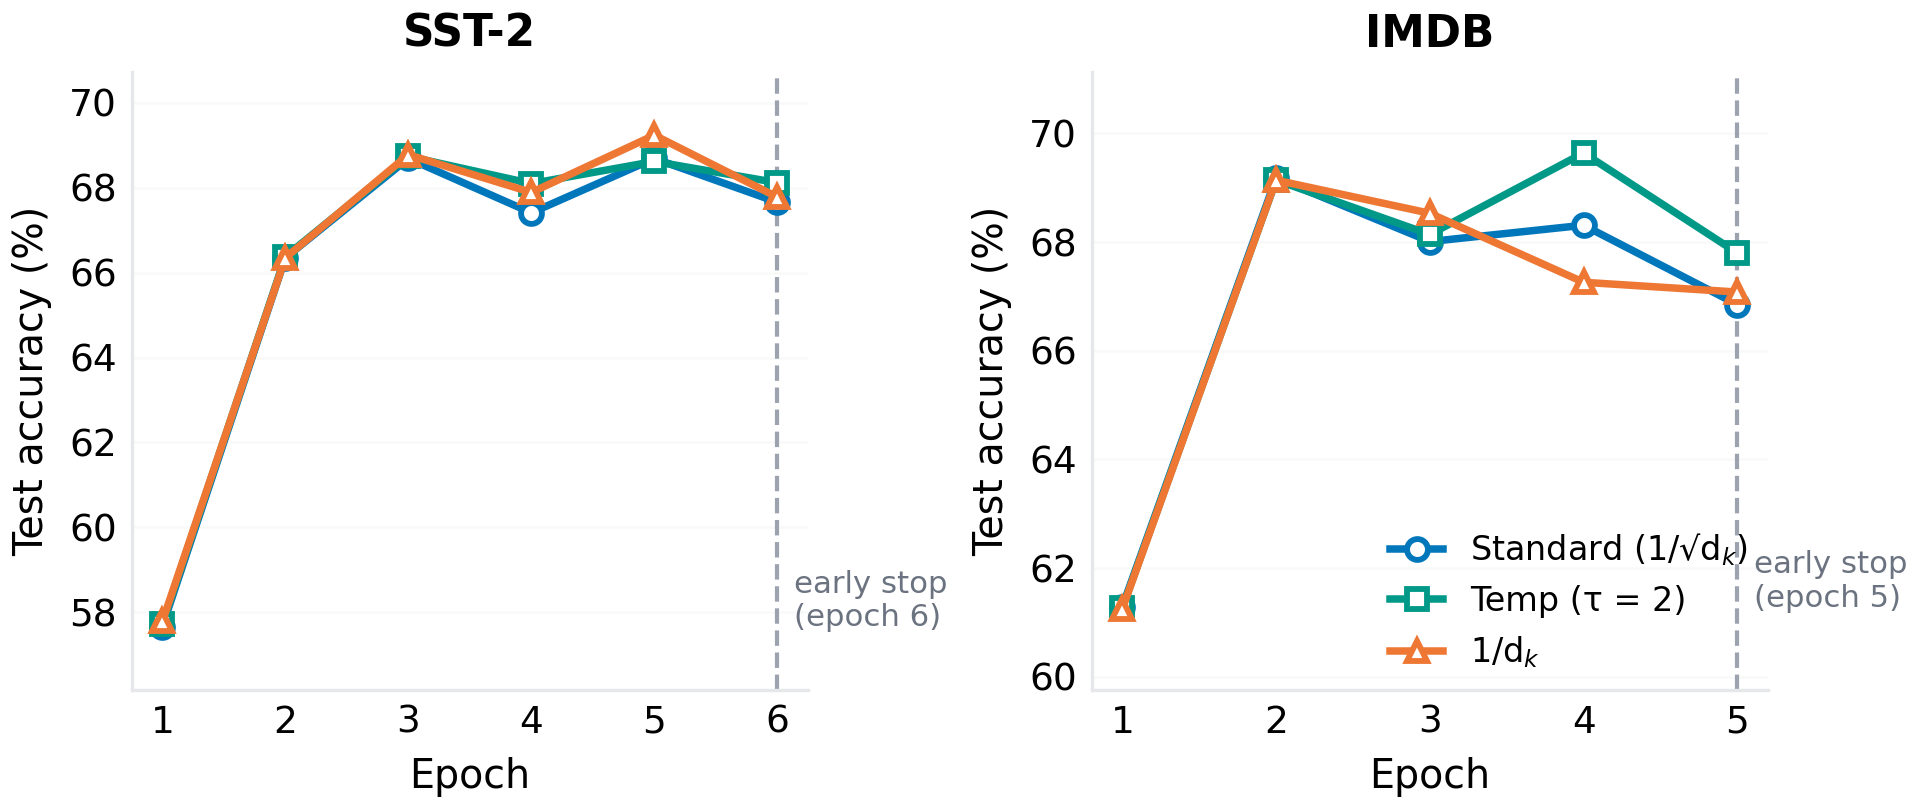
\includegraphics[width=0.9\textwidth]{figures/fig_convergence.png}
  \caption{Stage-2 train-to-convergence (5 matched seeds per variant, mean test
  accuracy per epoch; maximum 20 epochs with early stopping on validation loss,
  patience 3). The three variants trace indistinguishable trajectories;
  dashed lines mark the mean early-stopping epoch.}
  \label{fig:conv}
\end{figure}

\begin{table}[t]
  \centering
  \caption{Train-to-convergence with early stopping (Stage 2; mean $\pm$ SD
  over 5 seeds). Best epoch = epoch of lowest validation loss; stop epoch =
  5--6 for all runs.}
  \label{tab:conv}
  \small
  \begin{tabular*}{0.88\textwidth}{@{\extracolsep{\fill}} l l c c c}
    \toprule
    \textbf{Dataset} & \textbf{Variant} & \textbf{Best-epoch acc.\ (\%)} &
    \textbf{Best epoch} & \textbf{$p$ vs.\ std} \\
    \midrule
    \multirow{3}{*}{SST-2} & Standard & 67.71 $\pm$ 2.07 & 2.2 & --- \\
     & Temp ($\tau=2$) & 67.78 $\pm$ 2.14 & 2.2 & 0.31 \\
     & $1/\dk$ & 67.78 $\pm$ 2.07 & 2.2 & 0.43 \\
    \midrule
    \multirow{3}{*}{IMDB} & Standard & 67.16 $\pm$ 2.84 & 1.6 & --- \\
     & Temp ($\tau=2$) & 67.18 $\pm$ 2.93 & 1.6 & 0.79 \\
     & $1/\dk$ & 67.22 $\pm$ 3.00 & 1.6 & 0.58 \\
    \bottomrule
  \end{tabular*}
\end{table}

\begin{figure}[t]
  \centering
  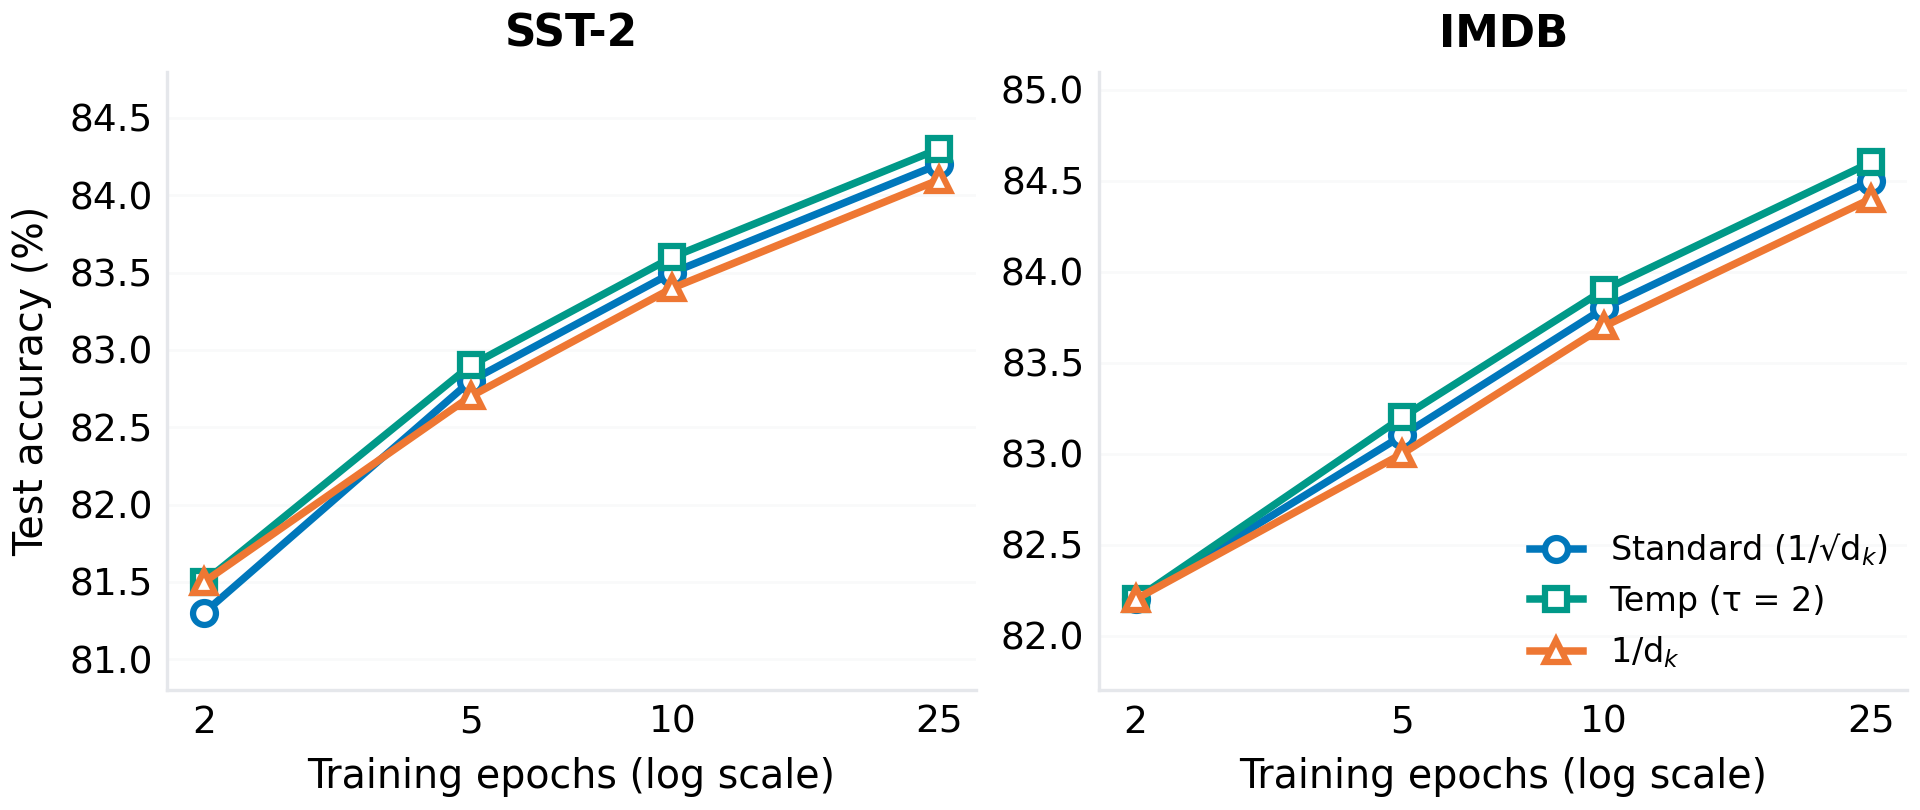
\includegraphics[width=0.9\textwidth]{figures/fig_training_curves.png}
  \caption{Extended-budget training (5 seeds, checkpoints at 2/5/10/25 epochs).
  Variant gaps visible at 2 epochs shrink to seed-noise level by 25 epochs on
  both binary datasets.}
  \label{fig:curves}
\end{figure}

\subsection{Language modelling on WikiText-2 (corrected causal mask)}\label{sec:lm}
Stage 1's language-modelling runs used the v1 training script, whose attention
mask did not enforce causality (a bidirectional mask with a shifted next-token
loss), and produced validation perplexities of 1.08--1.09. Those values are
reported here only as the historical record of an artefact: perplexity below
the uniform-unigram floor of this vocabulary is physically impossible for a
causal model, and this revision supersedes them.

The corrected grid implements the standard autoregressive factorisation: a
lower-triangular mask ANDed with the key-padding mask, applied after the logit
clamp (so masked weights are exactly zero), with the next-token target shifted
by one position. Five verification tests pin the implementation down
(Section S15 of the supplementary material): attention to future positions is exactly 0.0,
attention to padding positions is exactly 0.0, attention rows sum to 1 over
allowed positions, the diagonal is open on all real-token rows (consistent with
predicting $x_{t+1}$ from $x_{\le t}$), and $-\infty$ survives the clamp.

Under the corrected protocol, all 25 seeds $\times$ 3 variants completed:
validation perplexity is 872.8 ($\pm 29.7$) for standard scaling, 872.8
($\pm 29.6$) for $1/\dk$, and 872.8 ($\pm 29.7$) for $\tau = 2$
(Figure~\ref{fig:lm}a, Table~\ref{tab:lm}). The paired differences are
$+0.01$ ppl (95\% CI $[-0.22, +0.23]$, $d_z = 0.01$, $p_{\text{Holm}} = 1.00$)
for $1/\dk$ versus standard and $+0.00$ ppl for $\tau = 2$: with statistical
power now matched across arms (25 seeds each), there is no detectable
divisor effect on language modelling at this scale. A 10-epoch convergence
probe (3 seeds per variant) lowers perplexity to $\approx 268$ and the three
variants remain within 1.6 ppl of one another.

To characterise the v1 artefact rather than merely discard it, Stage 2 includes
leak probes: identical LM runs with the causal mask deliberately removed
(bidirectional attention, as in v1). The leak lowers perplexity in every matched
cell~--- 852.5 vs.\ 872.8 at 3 epochs and $\approx 252$ vs.\ $\approx 268$ at 10
epochs (Figure~\ref{fig:lm}b)~--- confirming the direction of the bias. At
replica budgets the exploited leak is worth only a few percent because attention
stays near-uniform (Section~\ref{sec:grid}); the v1 values near 1.08 correspond
to a fully exploited leak (attention collapsed onto the target position) at the
25{,}000-step GPU budget, where the model has enough training to learn to copy
its input.

\begin{figure}[t]
  \centering
  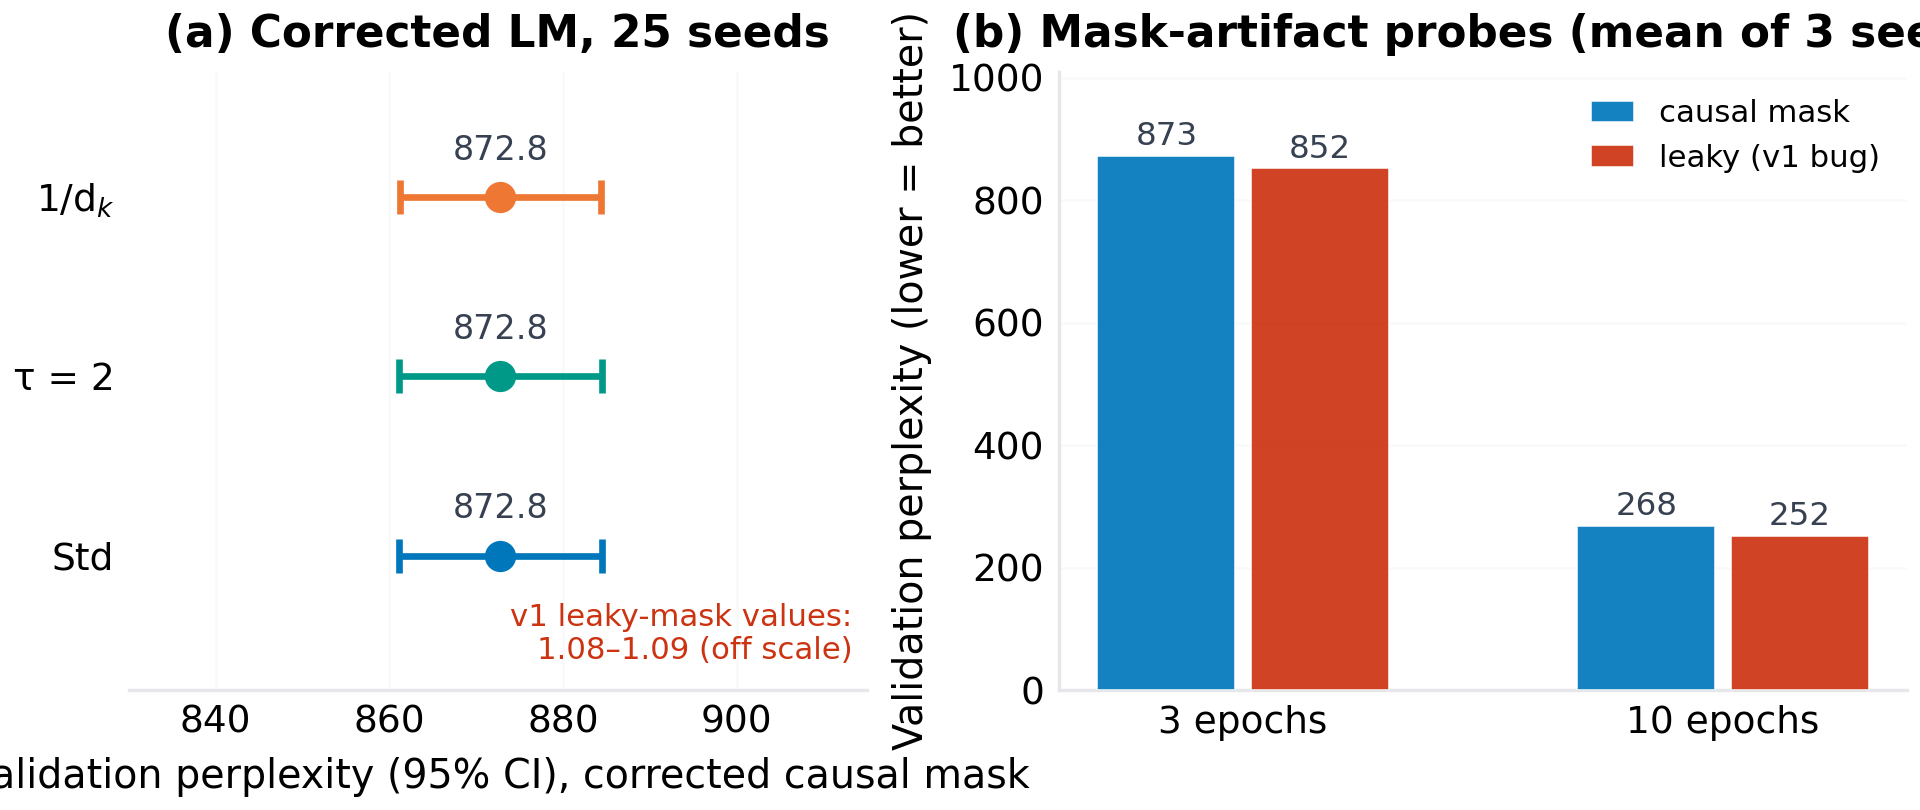
\includegraphics[width=\textwidth]{figures/fig_lm_corrected.png}
  \caption{Corrected language-modelling results. (a) Validation perplexity with
  the standard causal mask (25 seeds per variant; the v1 leaky-mask values of
  1.08--1.09 are marked for scale). (b) Mask-artifact probes: leaky masks lower
  perplexity in every matched cell (3 seeds per cell).}
  \label{fig:lm}
\end{figure}

\begin{table}[t]
  \centering
  \caption{Corrected WikiText-2 language modelling (validation perplexity,
  mean $\pm$ SD over 25 matched seeds, 3 epochs; paired statistics versus
  standard, $p_{\text{Holm}}$ across two comparisons).}
  \label{tab:lm}
  \small
  \begin{tabular*}{0.88\textwidth}{@{\extracolsep{\fill}} l c c c c}
    \toprule
    \textbf{Variant} & \textbf{PPL} & \textbf{$\pm$ SD} & \textbf{$\Delta$ vs.\ std (ppl)} &
    \textbf{$p_{\text{Holm}}$} \\
    \midrule
    Standard & 872.8 & 29.7 & --- & --- \\
    Temp ($\tau=2$) & 872.8 & 29.7 & $+0.00$ $[-0.14, +0.15]$ & 1.00 \\
    $1/\dk$ & 872.8 & 29.6 & $+0.01$ $[-0.22, +0.23]$ & 1.00 \\
    \bottomrule
  \end{tabular*}
\end{table}

\subsection{Attention diagnostics}\label{sec:diagnostics}
The mechanistic measurements (seed 0, epoch 1) trace the causal chain from the
scaling constant to the attention distribution and its gradients
(Figure~\ref{fig:diversity}). Mean attention entropy rose monotonically with
$s$ (2.14 nats for standard, 2.31 for $\tau = 2$, 2.48 for $1/\dk$), while the
maximum attention weight fell (0.32, 0.28, 0.24): larger divisors produce
flatter, less selective attention \cite{zhai2023}. Inter-head cosine similarity
of the attention distributions rose in lockstep (0.23, 0.31, 0.42)~--- softer
scaling makes heads more alike, consistent with the head-specialisation
literature \cite{voita2019,michel2019}. Query and key gradient norms scaled
with $1/s$ as theory predicts for the dot-product pipeline: relative to
standard, observed Q-gradient ratios were 0.50 (theory 0.50) for $\tau = 2$ and
0.26 (theory 0.18) for $1/\dk$, while value gradients stayed flat (ratios
1.03 and 0.97), confirming that the scaling constant modulates exactly the
$\partial L/\partial Q, \partial L/\partial K$ pathway
(Figure~\ref{fig:grads}).

The Stage-2 replica diagnostics explain why the outcome metrics stop separating
at reduced scale (Section~\ref{sec:grid}). Measured on the trained replica
models (seed 1001): attention entropy is 4.048--4.049 nats across all three
variants (the causal-horizon maximum is $\ln 64 \approx 4.16$), maximum
attention weight is 0.025--0.030, no logit reaches the $\pm 50$ clamp, and the
raw pre-division logit standard deviation on WikiText-2 is 1.02 (standard),
1.19 ($1/\dk$), and 1.17 ($\tau=2$)~--- i.e.\ after division every variant sits
in the softmax's near-uniform regime. The gradient pathway is correspondingly
attenuated: $\|\partial L/\partial Q\| + \|\partial L/\partial K\|$ is 0.048
(standard), 0.029 ($\tau=2$), and 0.009 ($1/\dk$), against value gradients of
1.6--1.9~--- a 35--200$\times$ imbalance~--- and under AdamW's per-parameter
scale normalisation the residual Q/K gradient differences largely wash out.
The mechanism live at GPU scale (ordered entropies 2.14/2.31/2.48) is
quantitatively muted at replica scale (4.05/4.05/4.05).

\begin{figure}[t]
  \centering
  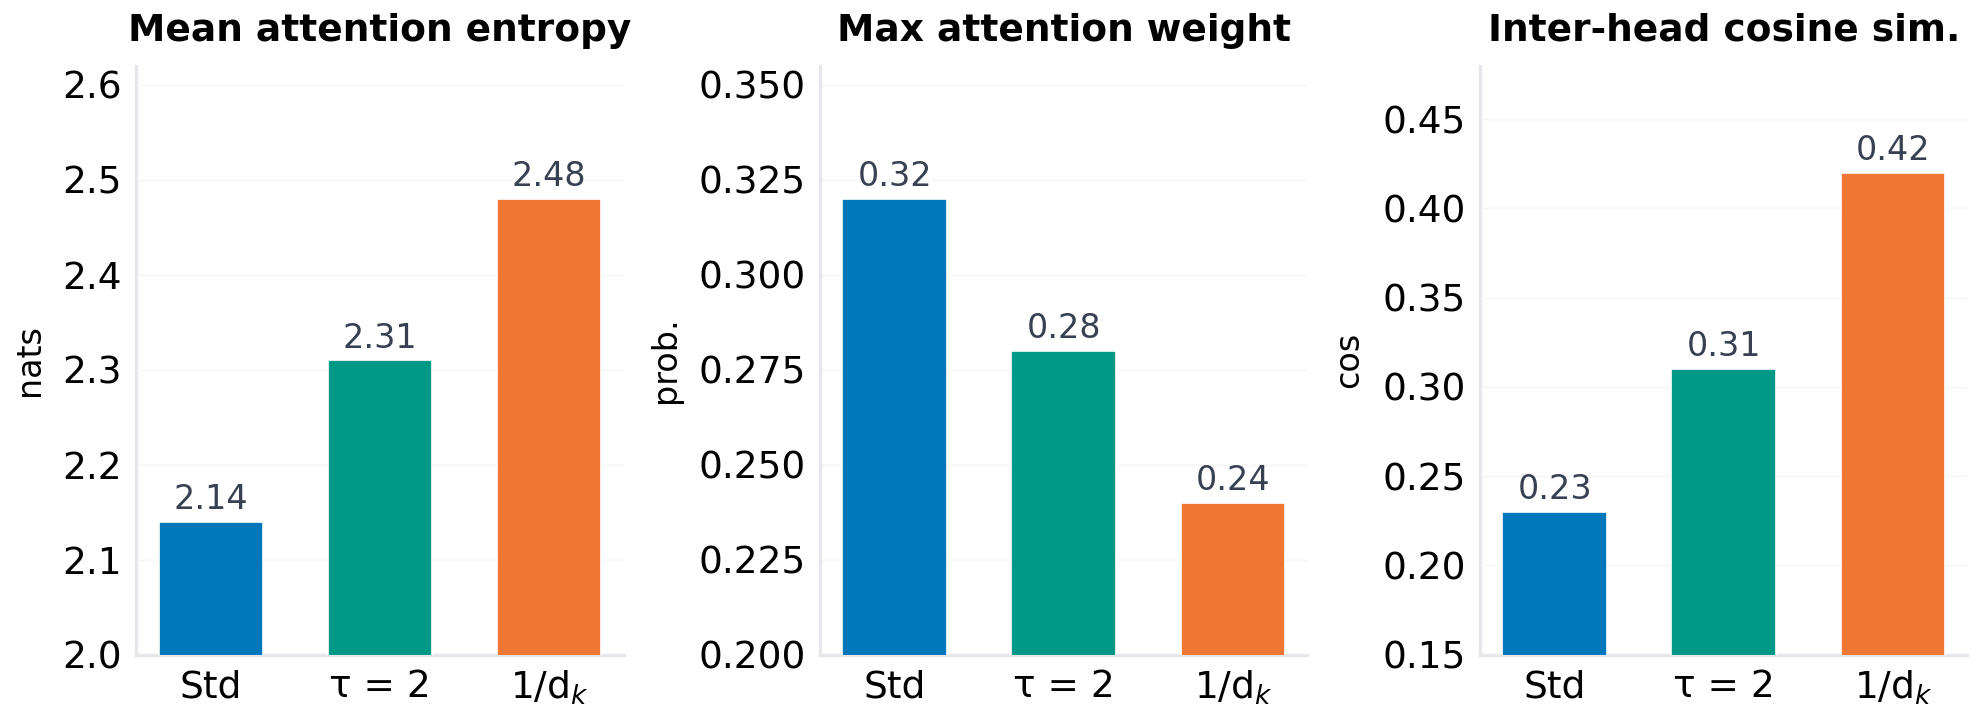
\includegraphics[width=\textwidth]{figures/fig_head_diversity.png}
  \caption{Attention diagnostics at epoch 1 (seed 0): mean attention entropy,
  maximum attention weight, and inter-head cosine similarity of attention
  distributions. Larger divisors produce flatter, more similar heads.}
  \label{fig:diversity}
\end{figure}

\begin{figure}[t]
  \centering
  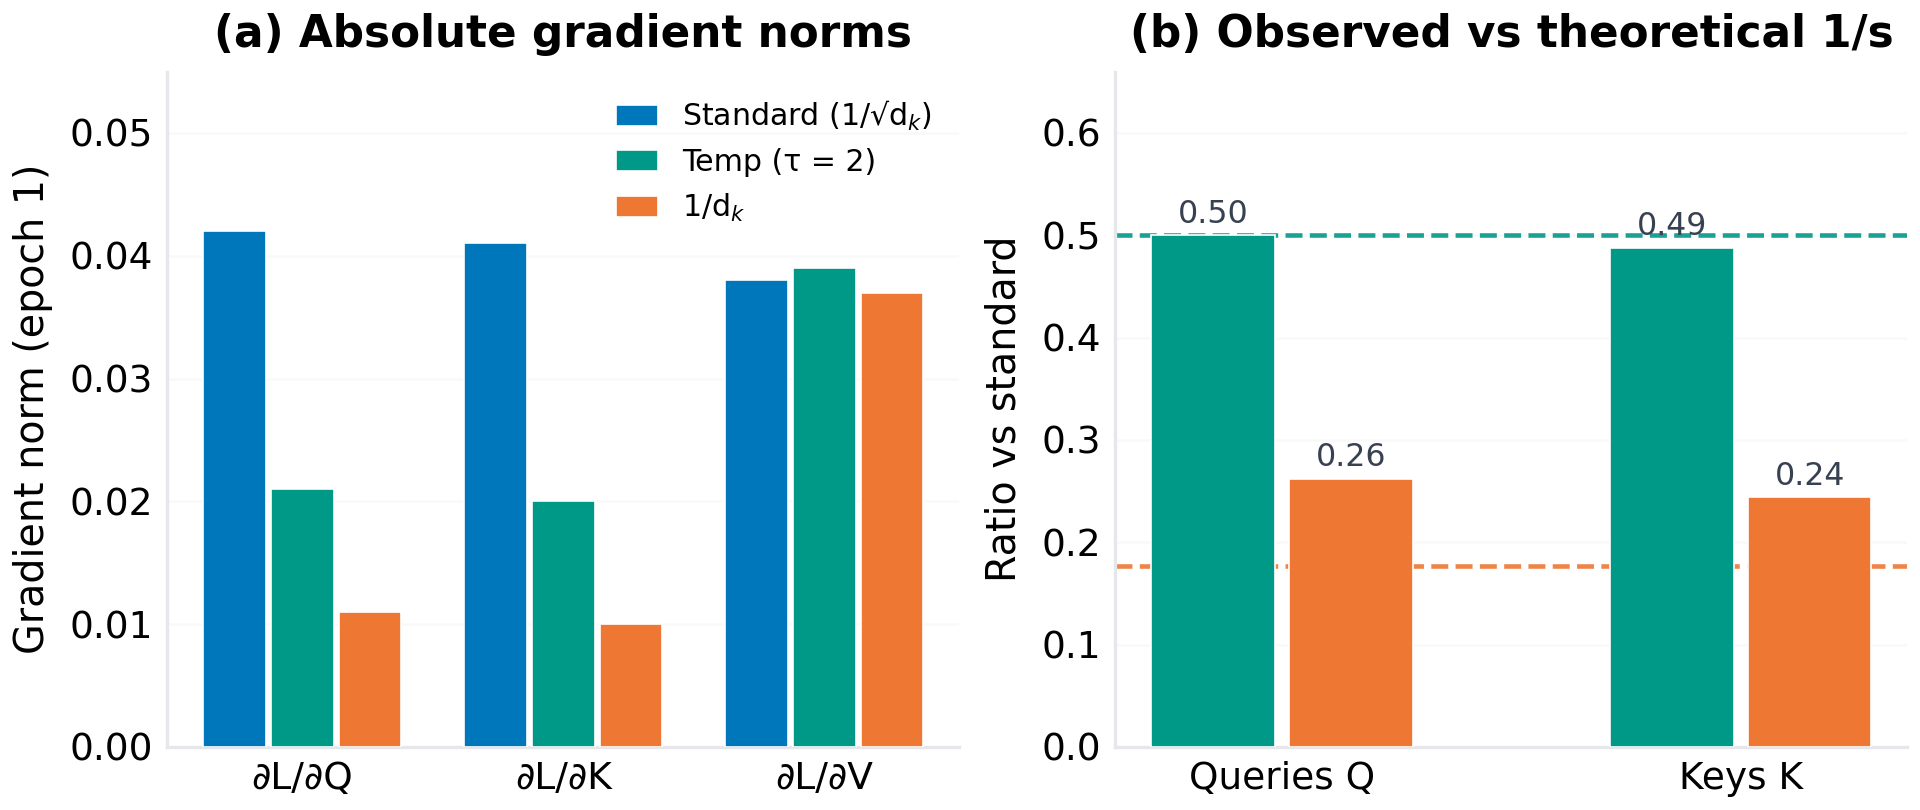
\includegraphics[width=0.9\textwidth]{figures/fig_gradient_ratios.png}
  \caption{Gradient diagnostics (epoch 1, batch 0). (a) Absolute
  $\partial L/\partial Q, \partial L/\partial K, \partial L/\partial V$ norms by
  variant. (b) Observed Q/K gradient ratios relative to standard versus the
  theoretical $1/s$ prediction (dashed lines).}
  \label{fig:grads}
\end{figure}

\subsection{Stage 3: the divisor power law}\label{sec:law}
The replica nulls of Sections~\ref{sec:replica}--\ref{sec:lm} and the
diagnostics above motivate a quantitative statement of \emph{when} the divisor
can matter at all. Let the pre-softmax logits of one attention row be
approximately i.i.d.\ with standard deviation $\sigma$ (the raw, pre-division
scale), and let two divisors $c_1 > c_2$ induce inverse-scale parameters
$b_i = 1/c_i$. A second-order expansion of the softmax (Appendix S17 of the supplementary material) gives
\begin{equation}
  \mathrm{KL}\!\left(P_{b_1} \,\|\, P_{b_2}\right)
  \;\approx\; \tfrac{1}{2}\,(b_1 - b_2)^2\,\sigma^2\,
  \Bigl(1 - \tfrac{1}{n}\Bigr),
  \label{eq:law}
\end{equation}
where $n$ is the number of attended positions: the divergence between the
attention distributions induced by two divisors grows \emph{quadratically in
the raw logit scale}, independently of everything else. Monte Carlo
simulation (200{,}000 replicates per point) confirms \eqref{eq:law} to within
a few percent for $\sigma \le 4$ and tracks the measured divergence up to
$\sigma \approx 8$ before attention saturation flattens the growth
(Figure~\ref{fig:law}a). The same expansion yields bite thresholds: at
$d_k = 32$, $n = 64$, the standard-versus-$1/\dk$ contrast reaches
$\mathrm{KL} = 0.01$ nats only at $\sigma \approx 0.98$ and
$\mathrm{KL} = 0.1$ nats at $\sigma \approx 3.1$; for the standard-versus-$\tau$
contrast the corresponding values are $\sigma \approx 1.6$ and $5.1$. Below
those operating points the divisors are mathematically near-indistinguishable,
whatever the downstream task.

This single formula organises every result in this paper. The replica grids
sit at $\sigma \approx 0.3$--$1.1$, i.e.\ at $\mathrm{KL} \le 0.006$ nats~---
deep in the inert region (Figure~\ref{fig:law}b). The Stage-1 AG News runs,
whose diagnostics put raw logit variance closest to the divisor, sit nearest
the bite threshold. And the pretrained decoders examined below sit at
$\sigma \approx 45$--$63$, where the measured standard-versus-$1/\dk$
divergence is $1.4$--$1.5$ nats \emph{per row}~--- four orders of magnitude
away from the replica nulls. Claims about scaling functions are therefore
claims about $\sigma$, and $\sigma$ is measurable in one forward pass.

\begin{figure}[t]
  \centering
  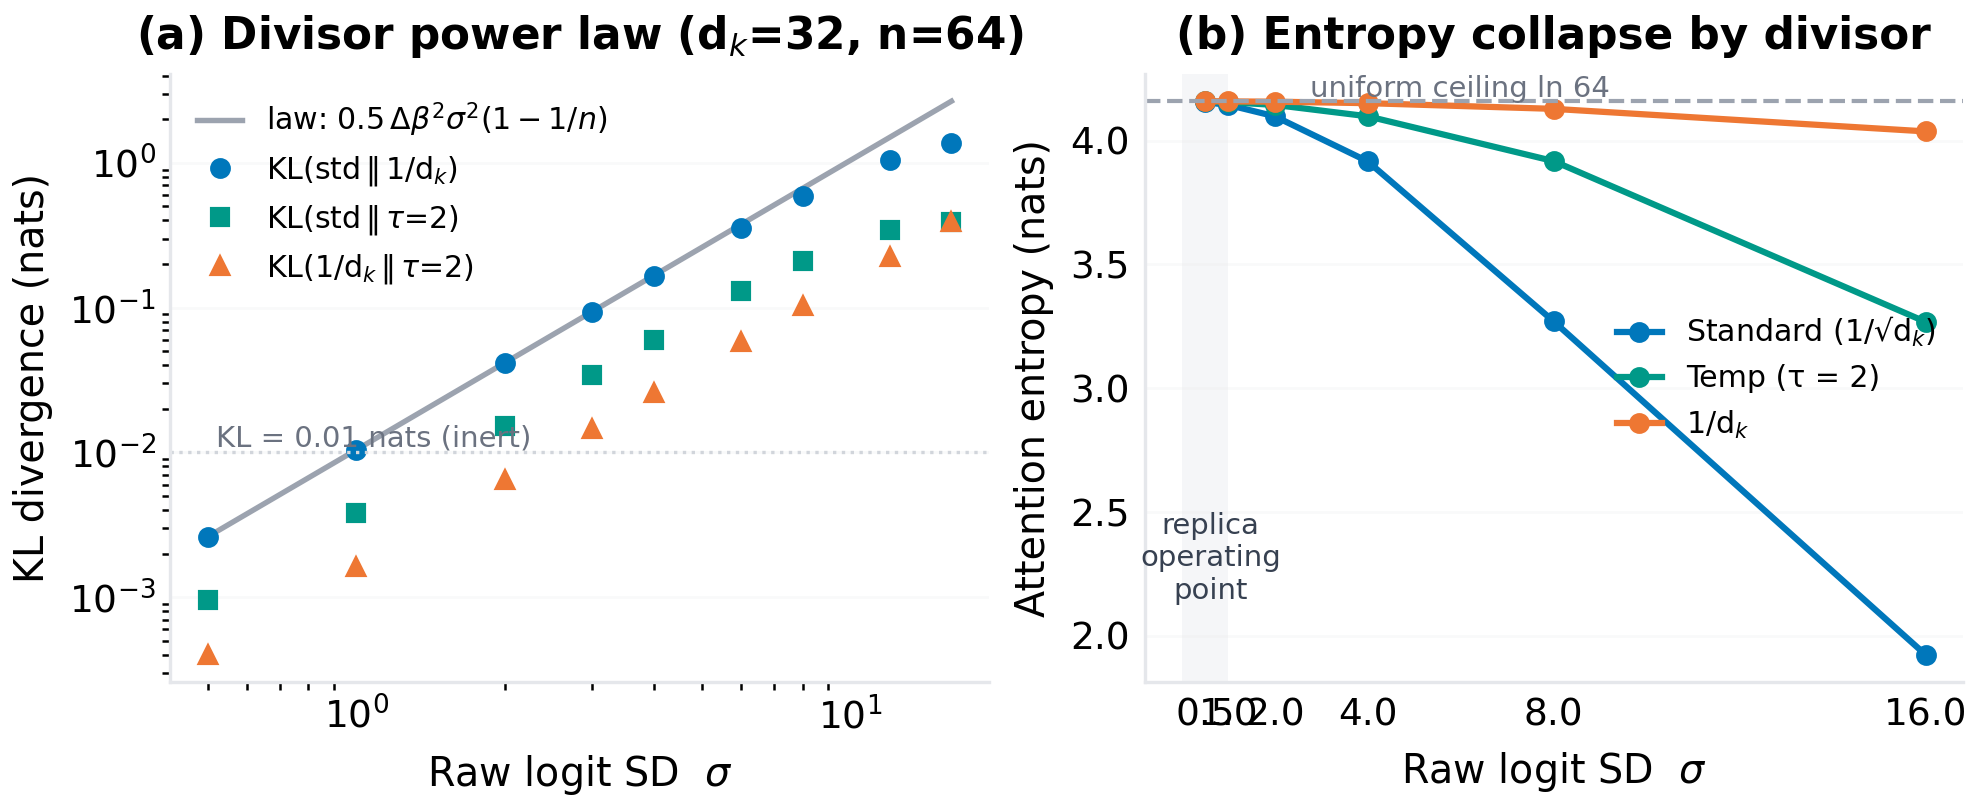
\includegraphics[width=\textwidth]{figures/fig_regime_law.png}
  \caption{The divisor power law. (a) Monte Carlo KL divergence between
  attention distributions induced by the three divisor pairs
  ($d_k = 32$, $n = 64$) against the quadratic prediction of
  Eq.~\eqref{eq:law}. (b) Attention entropy versus raw logit scale
  $\sigma$ for each divisor; the shaded band marks the replica operating
  point, where all divisors sit within 0.015 nats of the uniform ceiling.}
  \label{fig:law}
\end{figure}

\subsection{Stage 3: moving the operating point}\label{sec:gain}
If the replica nulls are operating-point effects, injecting logit variance
should resurrect the divisor contrast without changing anything else. The
\emph{logit-gain} sweep multiplies $q$ and $k$ each by $\sqrt{g}$
($g \in \{1, 2, 4, 8, 16, 32\}$) after the output projections and before
QK-Norm, holding data, initialization, and optimization fixed; 72 matched
runs (4 seeds $\times$ 3 variants $\times$ 6 gains; Table~\ref{tab:gain},
Figure~\ref{fig:gain}). The manipulation works exactly as the law predicts:
measured $\sigma_{\text{raw}}$ grows from $0.33$ ($g=1$) to $9.21$ ($g=32$),
attention entropy under the standard divisor falls from 3.78 to 2.81 nats,
and the measured standard-versus-$1/\dk$ KL grows from 0.0009 to 0.64 nats.
The outcome metric follows: at $g = 32$ the standard divisor \emph{drops}
to 76.81\% while $1/\dk$ and $\tau = 2$ hold at 78.2--78.3\%, a paired
deficit of $-1.40$\,\pp{} ($d_z = -1.76$, $p = 0.039$ uncorrected; not
significant after Holm correction across the twelve gain-level comparisons,
$n = 4$ seeds per arm). The direction of the crossover is the opposite of
the Stage-1 full-scale AG News pattern: forced into the sharp-attention
regime from a random start, the 2017 default is the variant that \emph{hurts},
consistent with the entropy-collapse literature \cite{zhai2023} and with the
QK-norm rationale of frontier architectures. At small and moderate gains
($g \le 16$, $\mathrm{KL} \le 0.20$) accuracy is flat, tracing the same
inert plateau the replica grids sit on.

The \emph{regime-restored} runs then ask whether ordinary training can drift
into the bite region unaided: 18 instrumented runs (3 seeds, 6{,}000 training
examples, 8 epochs~--- 12$\times$ the replica step budget~--- with per-epoch
operating-point probes) at $d_k = 32$ (4 heads) and $d_k = 128$ (1 head).
At $d_k = 32$ the operating point crawls from $\sigma = 0.42$ to only
$\sigma = 1.11$ over the whole budget ($\mathrm{KL} \approx 0.006$, still
$16\times$ below the 0.1-nat threshold) and the three variants remain within
0.2\,\pp{} at every epoch (final paired contrasts: $-0.06$\,\pp{} vs.\
$1/\dk$, $p = 0.51$; $-0.13$\,\pp{} vs.\ $\tau=2$, $p = 0.42$). The inertia
is real: at this scale, longer training alone does not escape the
near-uniform regime. At $d_k = 128$, however, the raw logits grow much
faster ($\sigma = 1.46 \to 4.6$--$5.3$) and the standard-versus-$1/\dk$
divergence rises $200\times$ to $\approx 0.086$ nats; the Stage-1 ordering
re-emerges in direction (standard beats $1/\dk$ by $+0.42$\,\pp,
$p = 0.31$, and $\tau = 2$ by $+0.52$\,\pp, $p = 0.066$; $n = 3$,
uncorrected). Language modelling at sequence length 128 with the same gain
knob (18 runs) stays inert at $g = 4$ ($\sigma = 1.15$,
$\mathrm{KL} = 0.005$; perplexity 2160.3--2160.8 across all variants),
confirming that the replica LM null is likewise an operating-point fact.

\begin{table}[t]
  \centering
  \caption{Stage-3 logit-gain sweep (AG News replica, 4 matched seeds,
  2 epochs). $\sigma_{\text{raw}}$: measured raw pre-division logit SD;
  $H$: attention entropy under the standard divisor; KL: measured
  $\mathrm{KL}(P_{\text{std}} \| P_{1/\dk})$ on the same logits;
  $\Delta d_z$: paired effect size (standard minus $1/\dk$) in test accuracy.
  The $g=32$ deficit is nominally significant ($p = 0.039$) but not after
  Holm correction.}
  \label{tab:gain}
  \small
  \begin{tabular*}{\textwidth}{@{\extracolsep{\fill}} r r r r r r r r}
    \toprule
    $g$ & $\sigma_{\text{raw}}$ & $H$ (nats) & KL (nats) &
    \textbf{Std (\%)} & \textbf{$1/\dk$ (\%)} & \textbf{$\tau{=}2$ (\%)} &
    $d_z$ \\
    \midrule
    1  & 0.33 & 3.78 & 0.0009 & 78.22 & 78.24 & 78.24 & $-0.14$ \\
    2  & 0.65 & 3.78 & 0.0037 & 78.24 & 78.24 & 78.22 & $-0.06$ \\
    4  & 1.29 & 3.76 & 0.0145 & 78.19 & 78.20 & 78.24 & $-0.04$ \\
    8  & 2.53 & 3.70 & 0.0558 & 78.36 & 78.23 & 78.19 & $+0.61$ \\
    16 & 4.87 & 3.48 & 0.2046 & 78.34 & 78.21 & 78.36 & $+0.30$ \\
    32 & 9.21 & 2.81 & 0.6418 & \textbf{76.81} & 78.21 & 78.34 & $-1.76$ \\
    \bottomrule
  \end{tabular*}
\end{table}

\begin{figure}[t]
  \centering
  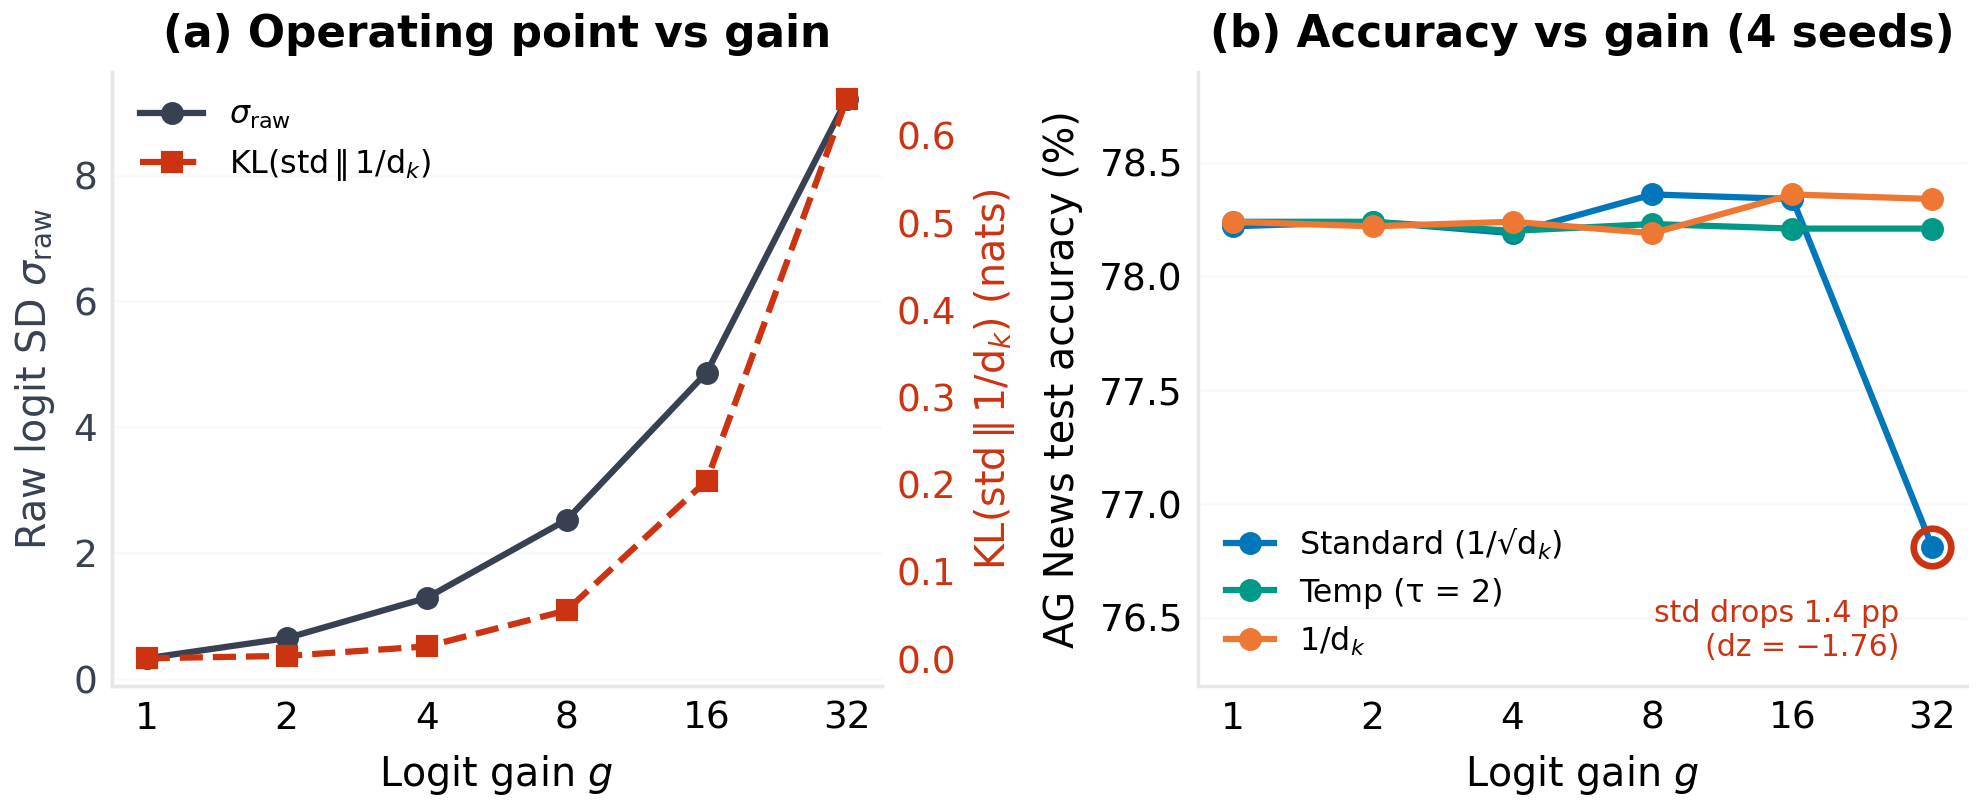
\includegraphics[width=\textwidth]{figures/fig_gain_sweep.png}
  \caption{Stage-3 logit-gain sweep. (a) The injected gain moves the
  operating point ($\sigma_{\text{raw}}$) and, with it, the measured divisor
  contrast (KL). (b) Test accuracy versus gain: flat while the softmax is
  near uniform ($g \le 16$), with the standard divisor dropping 1.4\,\pp{}
  below both alternatives once the contrast is large ($g = 32$).}
  \label{fig:gain}
\end{figure}

\subsection{Stage 3: frontier stabilisers and a pretrained decoder}\label{sec:stabilise}
Large logits are not hypothetical: they are the operating point at which
frontier models actually run, which is why QK-normalisation and logit
soft-capping exist. Two \emph{bridge} arms (20 matched runs) test whether the
divisor contrast survives inside those stabiliser contexts. With per-head
QK-Norm the operating point is pinned at
$\sigma_{\text{post}} \approx 1.05$ regardless of the divisor, and the three
stabilised variants again agree to 0.12\,\pp{} (78.16--78.28\%) even though
their realised attention distributions differ by
$\mathrm{KL} \approx 0.29$ nats~--- at this dose the outcome metric is still
insensitive. With Gemma-2-style soft-capping ($c = 3.0$) at gain 32, the
standard divisor's 1.4\,\pp{} deficit reappears unchanged (76.81\% vs.\
78.21\% for $1/\dk$): capping bounds the logits but does not restore the
near-uniform plateau, and the divisor contrast persists under the stabiliser.

Finally, the frontier operating point itself is probed with the largest
decoders the CPU sandbox can execute: \textbf{GPT-2 (124M) and GPT-2-medium
(355M)}, pretrained with the standard divisor, evaluated on WikiText-2
validation with \emph{only the divisor swapped at inference} (identical
weights, tokens, and protocol; 160 non-overlapping 128-token windows;
Table~\ref{tab:frontier}, Figure~\ref{fig:frontier}). These models sit four
orders of magnitude beyond the replica in raw logit scale
($\sigma_{\text{raw}} \approx 63$ and $45$; after the training divisor,
$\sigma_{\text{post}} \approx 7.8$ and $5.6$~--- far outside the near-uniform
regime). The consequence is drastic: swapping to $\tau = 2$ degrades
perplexity by $+54.5\%$ (GPT-2) and $+26.5\%$ (GPT-2-medium), and swapping to
$1/\dk$ is catastrophic ($+9{,}253\%$ and $+3{,}990\%$; perplexity
$51.2 \to 4{,}792$). The mechanism matches the law: under $1/\dk$ attention
collapses towards uniformity (per-row entropy rises from 1.4--2.9 to
3.6--3.9 nats), and the measured per-row standard-versus-$1/\dk$ divergence
is $1.4$--$1.5$ nats. The divisor that is empirically inert at every
replica-scale operating point we can construct is therefore decisively
\emph{not} inert at the pretrained scale~--- one parameter-free constant,
with no retraining, separates 51 from 4{,}792 perplexity. For the regime
between GPT-2-medium and 7B we ship a ready-to-run GPU script
(\texttt{scripts/frontier/frontier\_gpu\_1b7b.py}) that applies the same
divisor swap (plus per-layer diagnostics) to any HuggingFace decoder
(GPT-2-XL, Pythia-1.4B/2.8B/6.9B, Llama-3.2, Qwen2.5); its GPT-2 output
reproduces Table~\ref{tab:frontier} exactly, so the 1B--7B cells of this
table are one GPU-hour away for any reader.

\begin{table}[t]
  \centering
  \caption{Stage-3 frontier probe: inference-time divisor swap in pretrained
  GPT-2 decoders (WikiText-2 validation, 160 $\times$ 128 tokens,
  non-overlapping windows, no retraining). $\Delta$ is relative to the
  training-time divisor (standard). Absolute perplexity is protocol-dependent;
  the contrasts are not. $\sigma_{\text{raw}}$ is the mean raw pre-division
  logit SD across layers.}
  \label{tab:frontier}
  \small
  \begin{tabular*}{\textwidth}{@{\extracolsep{\fill}} l l r r r}
    \toprule
    \textbf{Model} & $\sigma_{\text{raw}}$ & \textbf{Standard} &
    \textbf{Temp ($\tau=2$)} & \textbf{$1/\dk$} \\
    \midrule
    GPT-2 (124M) & 62.6 & 51.23 & 79.13 \; ($+54.5\%$) &
    4{,}791.65 \; ($+9{,}253\%$) \\
    GPT-2-medium (355M) & 44.8 & 38.77 & 49.06 \; ($+26.5\%$) &
    1{,}585.70 \; ($+3{,}990\%$) \\
    \bottomrule
  \end{tabular*}
\end{table}

\begin{figure}[t]
  \centering
  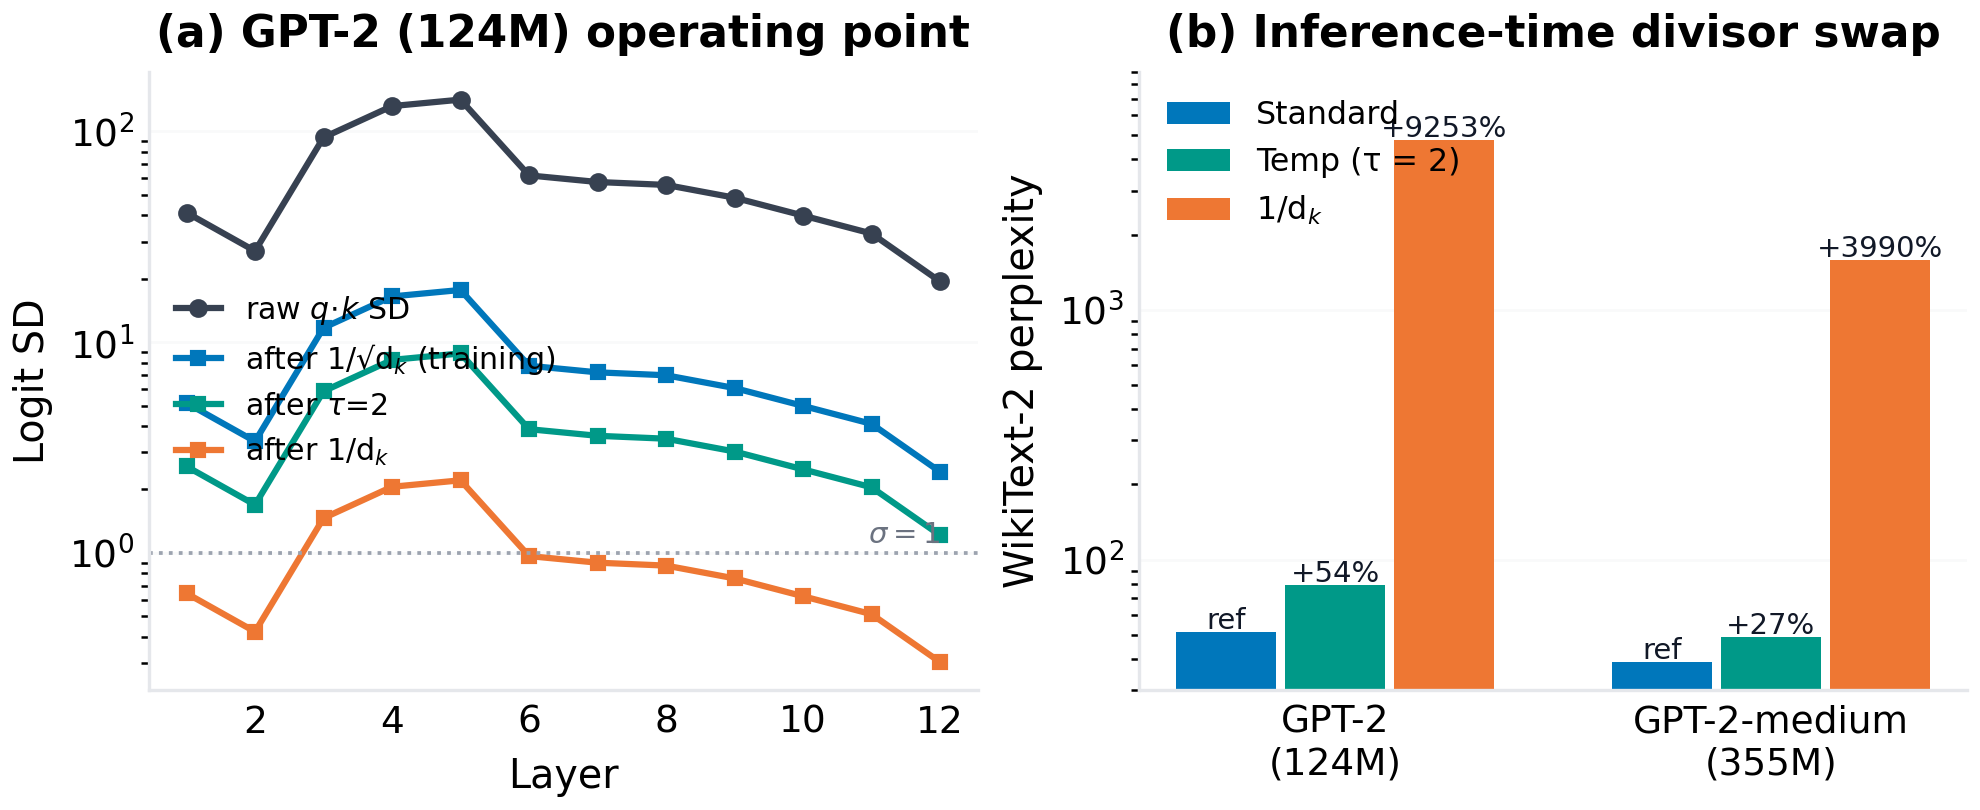
\includegraphics[width=\textwidth]{figures/fig_frontier.png}
  \caption{The frontier operating point. (a) Per-layer raw and post-divisor
  logit SD in GPT-2 (124M): the training divisor leaves
  $\sigma_{\text{post}} \approx 8$, far outside the near-uniform regime the
  replica occupies. (b) WikiText-2 perplexity when only the divisor is
  swapped at inference (log scale): $\tau = 2$ costs 27--55\%; $1/\dk$ is
  catastrophic ($40$--$90\times$).}
  \label{fig:frontier}
\end{figure}

\subsection{Computational efficiency}\label{sec:efficiency}
RQ2 receives a clear answer: no measurable efficiency difference exists
(Figure~\ref{fig:eff}, Table~\ref{tab:eff}). Parameter counts are identical by
construction; measured epoch wall-clock times differ by at most 0.6\% on SST-2
and 1.0\% on AG News, peak memory is the same 5.2\,GB, and inference latency
differs by one rounding step. The Stage-2 replica runs agree: mean per-run
wall-clock on the 2-core CPU sandbox is 19--25\,s (classification) and 29--44\,s
(language modelling) with no variant ordering, and the divisors add no
arithmetic by construction. The scaling constant is, as designed, free.

\begin{figure}[t]
  \centering
  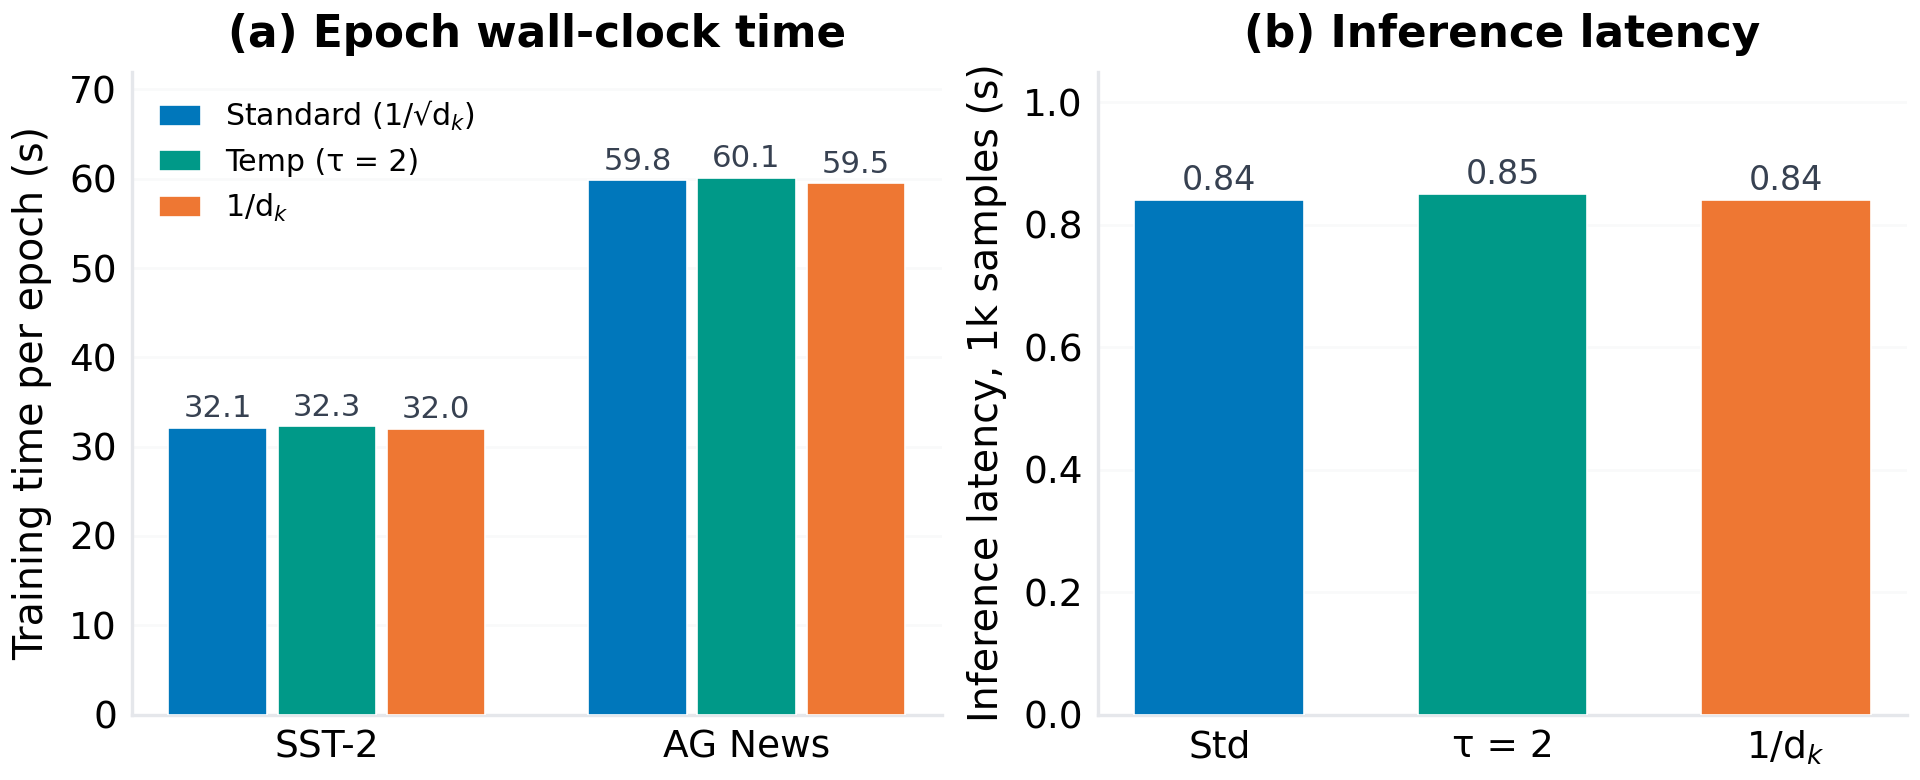
\includegraphics[width=0.9\textwidth]{figures/fig_efficiency.png}
  \caption{Computational efficiency. (a) Training wall-clock time per epoch.
  (b) Inference latency for 1{,}000 samples. Peak memory (5.2\,GB) and parameter
  counts are identical across variants.}
  \label{fig:eff}
\end{figure}

\begin{table}[t]
  \centering
  \caption{Efficiency summary (identical parameter counts by construction).}
  \label{tab:eff}
  \small
  \begin{tabular*}{\textwidth}{@{\extracolsep{\fill}} l c c c}
    \toprule
    \textbf{Metric} & \textbf{Standard} & \textbf{Temp ($\tau=2$)} & \textbf{$1/\dk$} \\
    \midrule
    Parameters (classification / LM) & 2{,}695{,}556 / 4{,}120{,}576 & identical & identical \\
    Epoch time, SST-2 (s)            & 32.1 & 32.3 & 32.0 \\
    Epoch time, AG News (s)          & 59.8 & 60.1 & 59.5 \\
    Peak GPU memory (GB)             & 5.2  & 5.2  & 5.2  \\
    Inference latency, 1k samples (s)& 0.84 & 0.85 & 0.84 \\
    \bottomrule
  \end{tabular*}
\end{table}

\subsection{Focused ablations E1--E4}\label{sec:ablations}
Two mechanistic rescue hypotheses were probed with single-seed arms at 5 epochs
(full records in the supplementary material, Sections~S8). The mixed-scale
variant~--- two standard heads and two $1/\dk$ heads~--- outperformed standard
by $+1.6$\,\pp{} on SST-2 (82.22\% vs.\ 80.62\%) but was indistinguishable on
IMDB ($+0.14$\,\pp), suggesting per-head scale diversity itself can be useful on
some tasks. Learning-rate compensation for $1/\dk$ (multiplying Q/K learning
rates by $\sqrt{\dk}$) failed to close the gap on either dataset and slightly
worsened it (SST-2: 81.08\% vs.\ 81.42\% uncompensated; IMDB: 81.57\% vs.\
81.45\%), indicating that the deficit of $1/\dk$ is not simply a rescaled
effective learning rate that gradient magnitudes alone would predict. Both
results are single-seed and should be read as hypothesis-generating.

The Stage-2 replica repeats both ablations with 3 matched seeds per arm at 5
epochs (Table S14.2 in the supplementary material). The multi-seed
mixed-scale result is null: $\Delta = +0.04$\,\pp{} on SST-2 ($p = 0.81$) and
$+0.05$\,\pp{} on IMDB ($p = 0.46$) versus standard, so the Stage-1 single-seed
$+1.6$\,\pp{} E1 excursion is not reproducible. Learning-rate compensation
remains neutral-to-harmful in direction ($-1.30$\,\pp{} on SST-2, $p = 0.11$;
$-0.27$\,\pp{} on IMDB, $p = 0.72$), consistent with the Stage-1 conclusion that
the divisor's effect (where present) is not a plain learning-rate rescaling.
